%!TEX root = ../dokumentation.tex

\chapter{Training und Evaluation eines Klassifikationsmodells} \label{ch:crispDm_2}

Dieses Kapitel gliedert sich in drei Abschnitte: das Training von diversen Klassifikationsmodellen, die Evaluation in Form von weiteren Experimenten und einer Diskussion und abschließend die Bereitstellung eines Modells.

\section{Training} \label{sec:modeling}

% Länge von falsch klassifizierten Einträgen analysieren

Auf Basis der bereinigten Datensätze werden im folgenden Abschnitt diverse Klassifikationsmodelle trainiert. Dies umfasst Baseline-Modelle mit \ac{BoW} und \ac{TF-IDF}, als auch neuronale Netze, die zusätzlich auf komprimierten Worteinbettungen trainiert werden. Ferner wird mit \ft und \ac{BERT} Modellen trainiert.

Grundlegend wird jedes Modell separat auf jedem Datensatz (Tweets, Reden, Wahlprogramme) trainiert. Im folgenden referenzieren wir darauf als in-domain. Modelle, die es durch ihren Ressourcenbedarf (Speicher und Rechenkapazität) zulassen, werden ebenfalls auf dem kommutierten Datensatz trainiert. 

% TODO: evtl. zu Beginn Metrik (Makro F1) einmal erklären und begründen + unabalanced / balanced inkl. warum undersampling

Wie \autoref{tab:countPerDatasetAfterCleaning} zeigt, sind die Klassen innerhalb der einzelnen Datensätze nicht ausgeglichen. Dies kann zu einem Bias hin zur am stärksten vertretenen Klasse führen. Zusätzlich zu den unbalancierten Daten werden die Klassen der Datensätze ebenfalls mit Unterabtastung (engl. undersampling) angeglichen. Als Metrik wird der Makro \(F_1\) Score verwendet. Dieser ergibt sich aus dem ungewichteten Durchschnitt der \(F_1\) Werte aller Klassen.

Für das Training der Baseline-Modelle sowie neuronalen Netze steht ein MacBook Pro mit dem Apple M1 Pro Prozessor und \num{8} Kernen zur Verfügung. Zudem bietet das MacBook \SI{16}{\giga\byte} an \ac{RAM} und eine \ac{GPU} mit \num{14} Kernen. Jegliche Trainings mit \ft oder \ac{BERT} erfolgen auf einem Computer mit einer Intel Xeon E3-1231 v3 \ac{CPU} mit \num{4} Kernen und \num{8} Threads. Außerdem verfügt der Computer über \SI{16}{\giga\byte} an \ac{RAM} und einer Nvidia GeForce GTX 1070 mit \SI{8}{\giga\byte} an \ac{GDDR5} Speicher.

\subsection{Baseline} \label{subsec:baseline}

Als ersten Ansatz zum Training eines Klassifikationsmodells werden -- als \enquote{Baseline} -- simple \ac{ML}-Verfahren auf der Basis von kontextunabhängigen Textrepräsentationsformen verwendet. Dabei werden die Trainings-Daten in Form von Text zuerst mittels \ac{BoW} als auch \ac{TF-IDF} vektorisiert, um als Input für ein Klassifikationsverfahren genutzt werden zu können.

Die Transformation der Eingabedaten resultiert in einer Matrix der Größe \(N \times V\), mit \(N\) als Anzahl der Datenpunkte und \(V\) der Größe des Vokabulars beziehungsweise der Anzahl aller einzigartigen Wörter im gesamten Datensatz. Das Vokabular wird im Folgenden auf die \num{50000} im Datensatz am meisten vorkommenden Wörter begrenzt. Dadurch wird vermieden, dass die Matrix zu groß wird und der \ac{RAM} auf dem genutzten Computer nicht ausreicht. Die zweite Dimension, die Anzahl an Einträgen eines Datensatzes, muss für die Tweets auf \num{125000} begrenzt werden. Bei der Beurteilung der Ergebnisse sollte berücksichtigt werden, dass daher nur gut ein Drittel der zur Verfügung stehenden Tweets bei auf \ac{BoW} oder \ac{TF-IDF} basierenden Ansätzen zum Training verwendet werden kann.

Es werden Wörter miteinbezogen, die in maximal \SI{20}{\percent} der Einträge vorkommen (\(max\_df = \num{0.2}\)). Die Python-Bibliothek \sk, die für die Vektorisierung und das Trainieren der Baseline-Modelle verwendet wird, bietet ebenfalls die Möglichkeit, nicht nur einzelne Wörter (1-grams) zur Repräsentation zu nutzen, sondern beliebige n-grams. Diese Option wird nicht genutzt (\(ngram\_range = (\num{1}, \num{1})\)), weil -- wie bereits angesprochen -- die Dimension der transformierten Matrix sonst zu groß werden würde. Außerdem stellt \ft eine ähnliche Methode bereit.

\sk bietet eine Reihe von Klassifikations-Algorithmen, die zusätzlich zur binären Klassifikation ebenfalls mehrere Klassen unterstützt \autocite{noauthor_112_nodate}. Hervorgehend aus den Experimenten erreichen Multinomial \ac{NB} sowie Lineare \ac{SVC} die beste Performance. Andere Modelle erreichen einen deutlich geringeren \(F_1\) Score\footnote{\texttt{KNeighborsClassifier}, \texttt{DecisionTreeClassifier} und \texttt{ExtraTreeClassifier}} oder trainieren wesentlich länger\footnote{\texttt{LogisticRegression}, \texttt{GradientBoostingClassifier} und \texttt{RandomForestClassifier}}.

Für die beiden gewählten Modelle sowie die Vektorisierung durch \ac{BoW} und \ac{TF-IDF} wird eine Hyperparameteroptimierung durch eine Rastersuche in \sk ausgehend von den Standardparametern durchgeführt. Dadurch ergibt sich eine Erhöhung der maximal durchzuführenden Iterationen bei der Linearen \ac{SVC} (\(max\_iter = \num{2000}\)) sowie die bereits dargestellte Konfiguration der Vektorisierung.
    
{\footnotesize
\begin{longtblr}[caption={Macro \(F_1\) Score für Lineare \ac{SVC}}, label={tab:overviewScoresBaselineSvc}, note{$\dag$}={Aufgrund von beschränkten Rechenressourcen zum Training wird der Datensatz auf \num{125000} zufällig ausgewählte Einträge beschränkt.}, remark{Parameter} = {\(max\_df = \num{0.2}\), \(ngram\_range = (\num{1}, \num{1})\), \(max\_iter = \num{2000}\)}]{hline{1, 3, Z} = {1pt}, rowhead = 2, colspec={l*{4}{Q[si={table-format=1.2},c]}}, row{1-2}={guard,font=\bfseries,l}}
     & \SetCell[c=2]{c} BoW & & \SetCell[c=2]{c} TF-IDF & \\
    \cline{2-5}
    Datensatz & Unbalanced & Balanced & Unbalanced & Balanced \\

    Tweets\TblrNote{$\dag$} & 0.50 & 0.49 & \textbf{\num{0.54}} & 0.52 \\
    Wahlprogramme & 0.50 & 0.47 & \textbf{\num{0.55}} & 0.51 \\
    Reden & 0.62 & 0.59 & \textbf{\num{0.66}} & 0.63 \\
\end{longtblr}
}

\autoref{tab:overviewScoresBaselineSvc} stellt die Ergebnisse des Trainings der Linearen \ac{SVC} auf allen drei Datensätzen einzeln und je auf Basis von \ac{BoW} und \ac{TF-IDF} dar. Als Metrik dient der Makro \(F_1\) Score. Das Training wurde sowohl auf dem unbalancierten (\enquote{balanced}) als auch auf einem durch Undersampling balancierten Datensatz mit gleicher Verteilung der Klassen (\enquote{unbalanced}) durchgeführt.

Auf jeden Datensatz erreicht \ac{TF-IDF} auf dem unbalancierten Datensatz den höchsten \(F_1\) Score. Der Tweet-Datensatz erreicht mit \num{0.54}, knapp hinter den Wahlprogrammen mit \num{0.55}, den schlechtesten Wert. Das Training auf den Reden erreicht einen deutlich bessere Score von \num{0.66}. Das Balancieren der Datensätze sinkt das Ergebnis jeweils um \numrange{0.2}{0.04}. \ac{BoW} schneidet konstant um \numrange{0.03}{0.05} Punkte schlechter ab als \ac{TF-IDF}.

{\footnotesize
\begin{longtblr}[caption={Makro \(F_1\) Score für Multinomial \ac{NB}}, label={tab:overviewScoresBaselineNb}, note{$\dag$}={Aufgrund von beschränkten Rechenressourcen zum Training wird der Datensatz auf \num{125000} zufällig ausgewählte Einträge beschränkt.}, remark{Parameter} = {\(max\_df = \num{0.2}\), \(ngram\_range = (\num{1}, \num{1})\)}]{hline{1, 3, Z} = {1pt}, rowhead = 2, colspec={l*{4}{Q[si={table-format=1.2},c]}}, row{1-2}={guard,font=\bfseries,l}}
     & \SetCell[c=2]{c} BoW & & \SetCell[c=2]{c} TF-IDF & \\
    \cline{2-5}
    Datensatz & Unbalanced & Balanced & Unbalanced & Balanced \\

    Tweets\TblrNote{$\dag$} & \textbf{\num{0.53}} & 0.52 & 0.52 & 0.51 \\
    Wahlprogramme & \textbf{\num{0.51}} & 0.49 & 0.24 & 0.50 \\
    Reden & \textbf{\num{0.61}} & 0.60 & 0.14 & 0.60 \\
\end{longtblr}
}

Die gleichen Trainings werden zudem mit Multinomial \ac{NB} durchgeführt. Dazu stellt \autoref{tab:overviewScoresBaselineNb} die Ergebnisse in gleicher Form dar. Anders als zuvor führt die Text-Vektorisierung mittels \ac{BoW} bei allen Datensätzen zu dem besten \(F_1\) Score. Die Wahlprogramme erreichen mit \num{0.51} den geringsten Wert. Der Tweet-Datensatz erreicht \num{0.53} und die Reden liefern \num{0.61} das beste Ergebnis. Auf balancierten Daten schneidet \ac{BoW} leicht schlechter ab. Mit \ac{TF-IDF} lässt sich für die unbalancierten Tweets ein ähnlich hoher \(F_1\) Score von \num{0.52} erreicht. Im Gegensatz zu \ac{BoW} fällt dieser für die unbalancierten Wahlprogramme und Reden aber auf \numrange{0.14}{0.24}. Auf den balancierten Datensätzen tritt diese Anomalie nicht auf. \ac{BoW} und \ac{TF-IDF} erreichen auf diesen nahezu identische Werte.

Die in \autoref{tab:overviewScoresBaselineSvc} und \autoref{tab:overviewScoresBaselineNb} dargestellten Ergebnisse betrachten jeweils mit dem Makro \(F_1\) Score einen gewichteten Durchschnitt zwischen den Ergebnissen für die einzelnen klassifizierten Parteien. Im Folgenden soll anhand der in \autoref{fig:confusionMatrixBaseline} dargestellten Konfusionsmatrizen genauer untersucht werden, welche Parteien besonders gut erkannt werden können und zwischen welchen Parteien viele Verwechslungen auftreten. Dabei wird auf die Ergebnisse des besten Baseline-Modells, der Linearen \ac{SVC} mit \ac{TF-IDF}, zurückgegriffen.
 
\begin{figure}[H]
    \centering
    \begin{subfigure}{0.49\textwidth}
        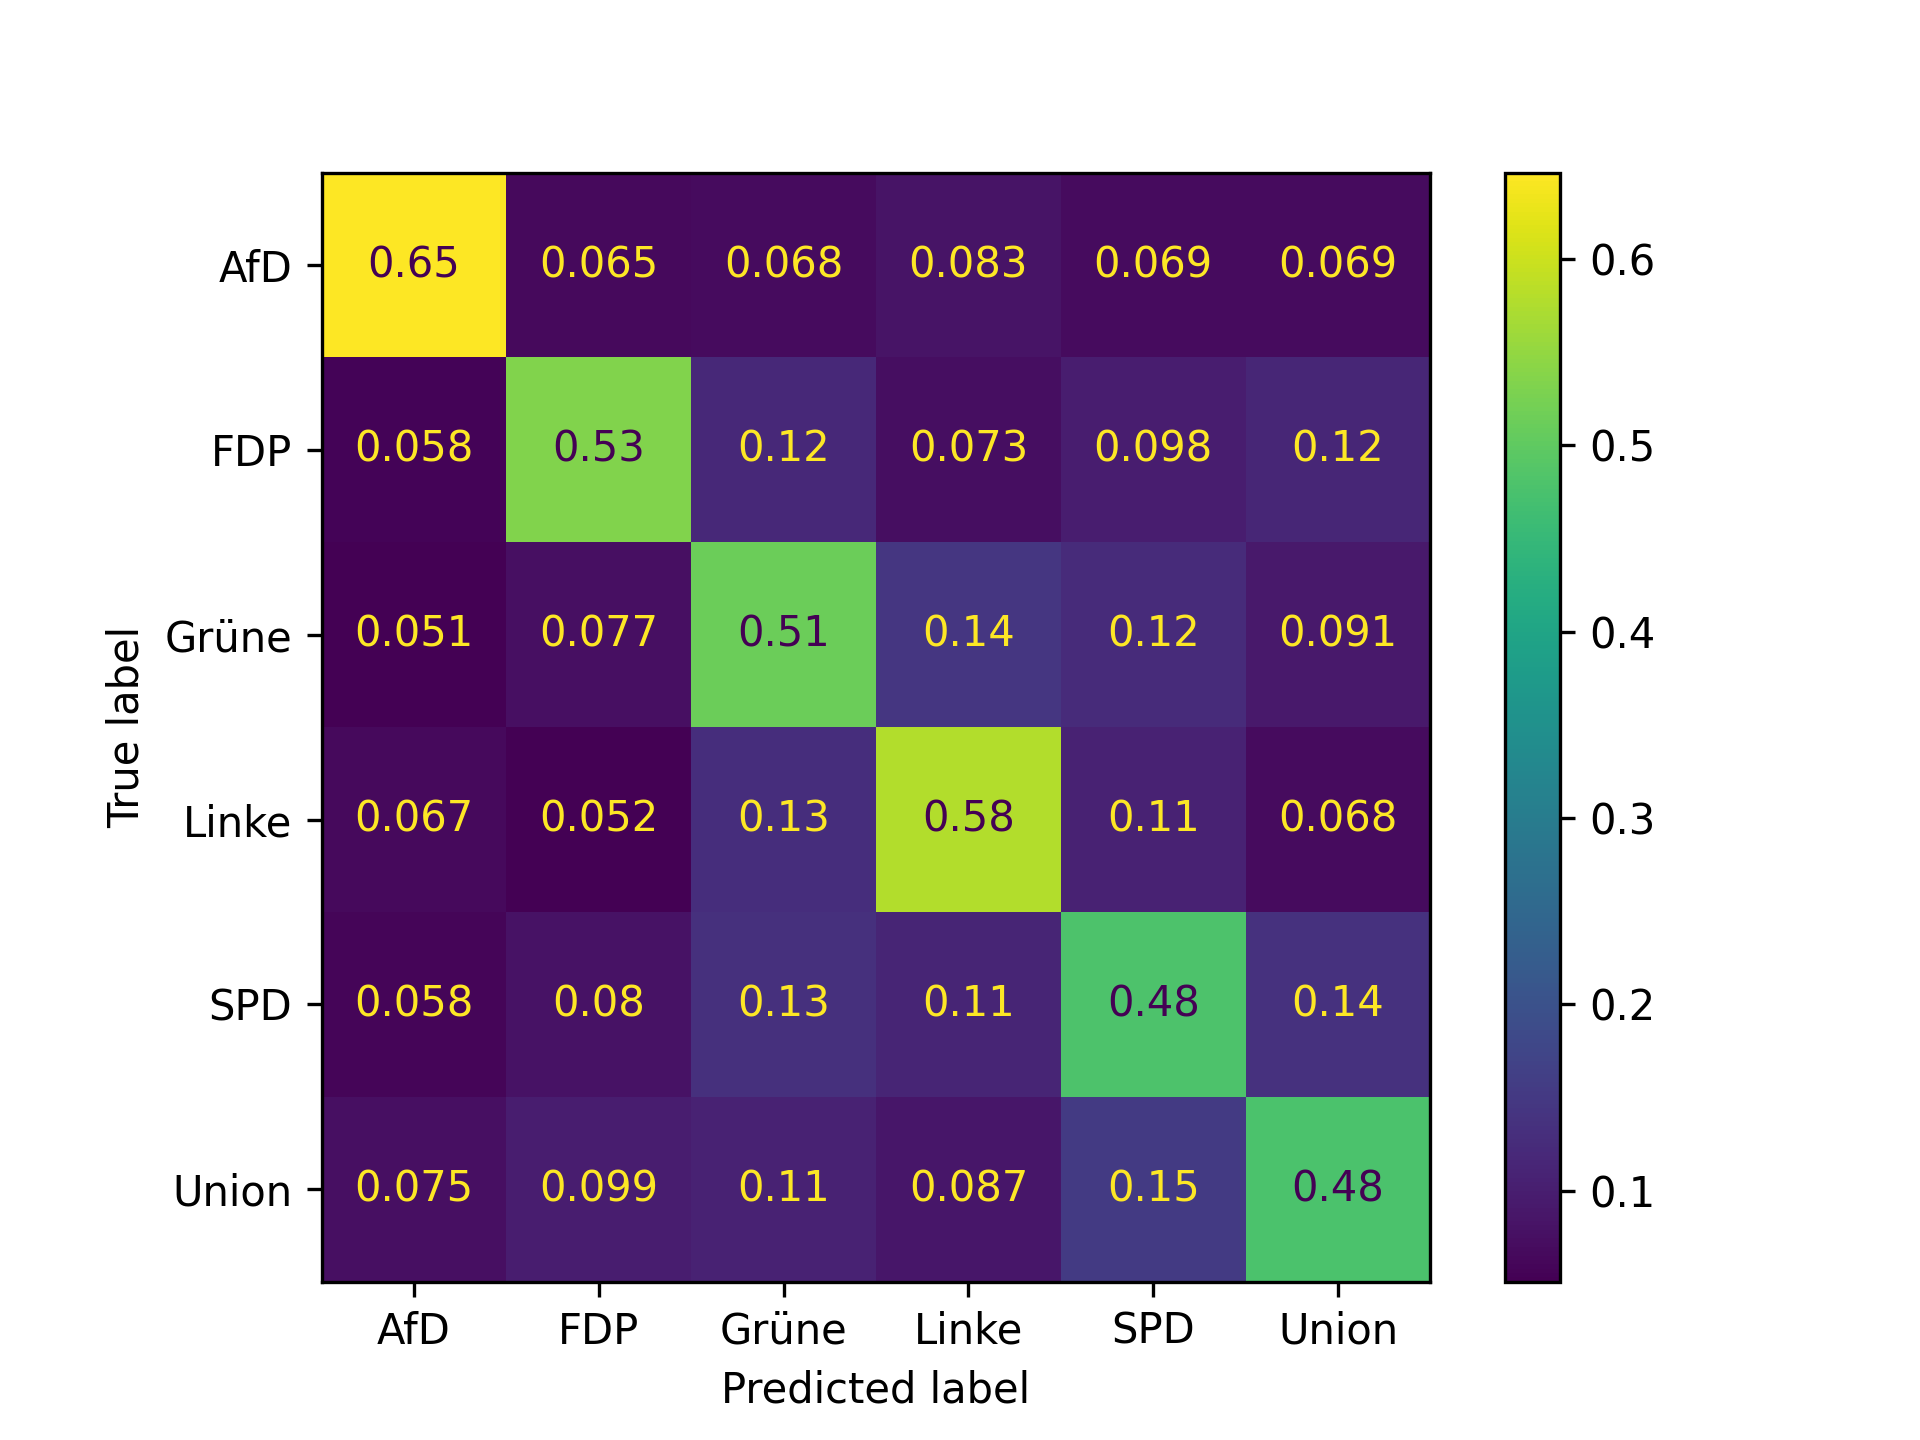
\includegraphics[width=\textwidth]{data/images/modeling/baseline/tweets_confusion_matrix.png}
        \caption{Tweets (\(N=\num{125000}\))}
        \label{sfig:confusionMatrixBaselineTweets}
    \end{subfigure}
    \hfill
    \begin{subfigure}{0.49\textwidth}
        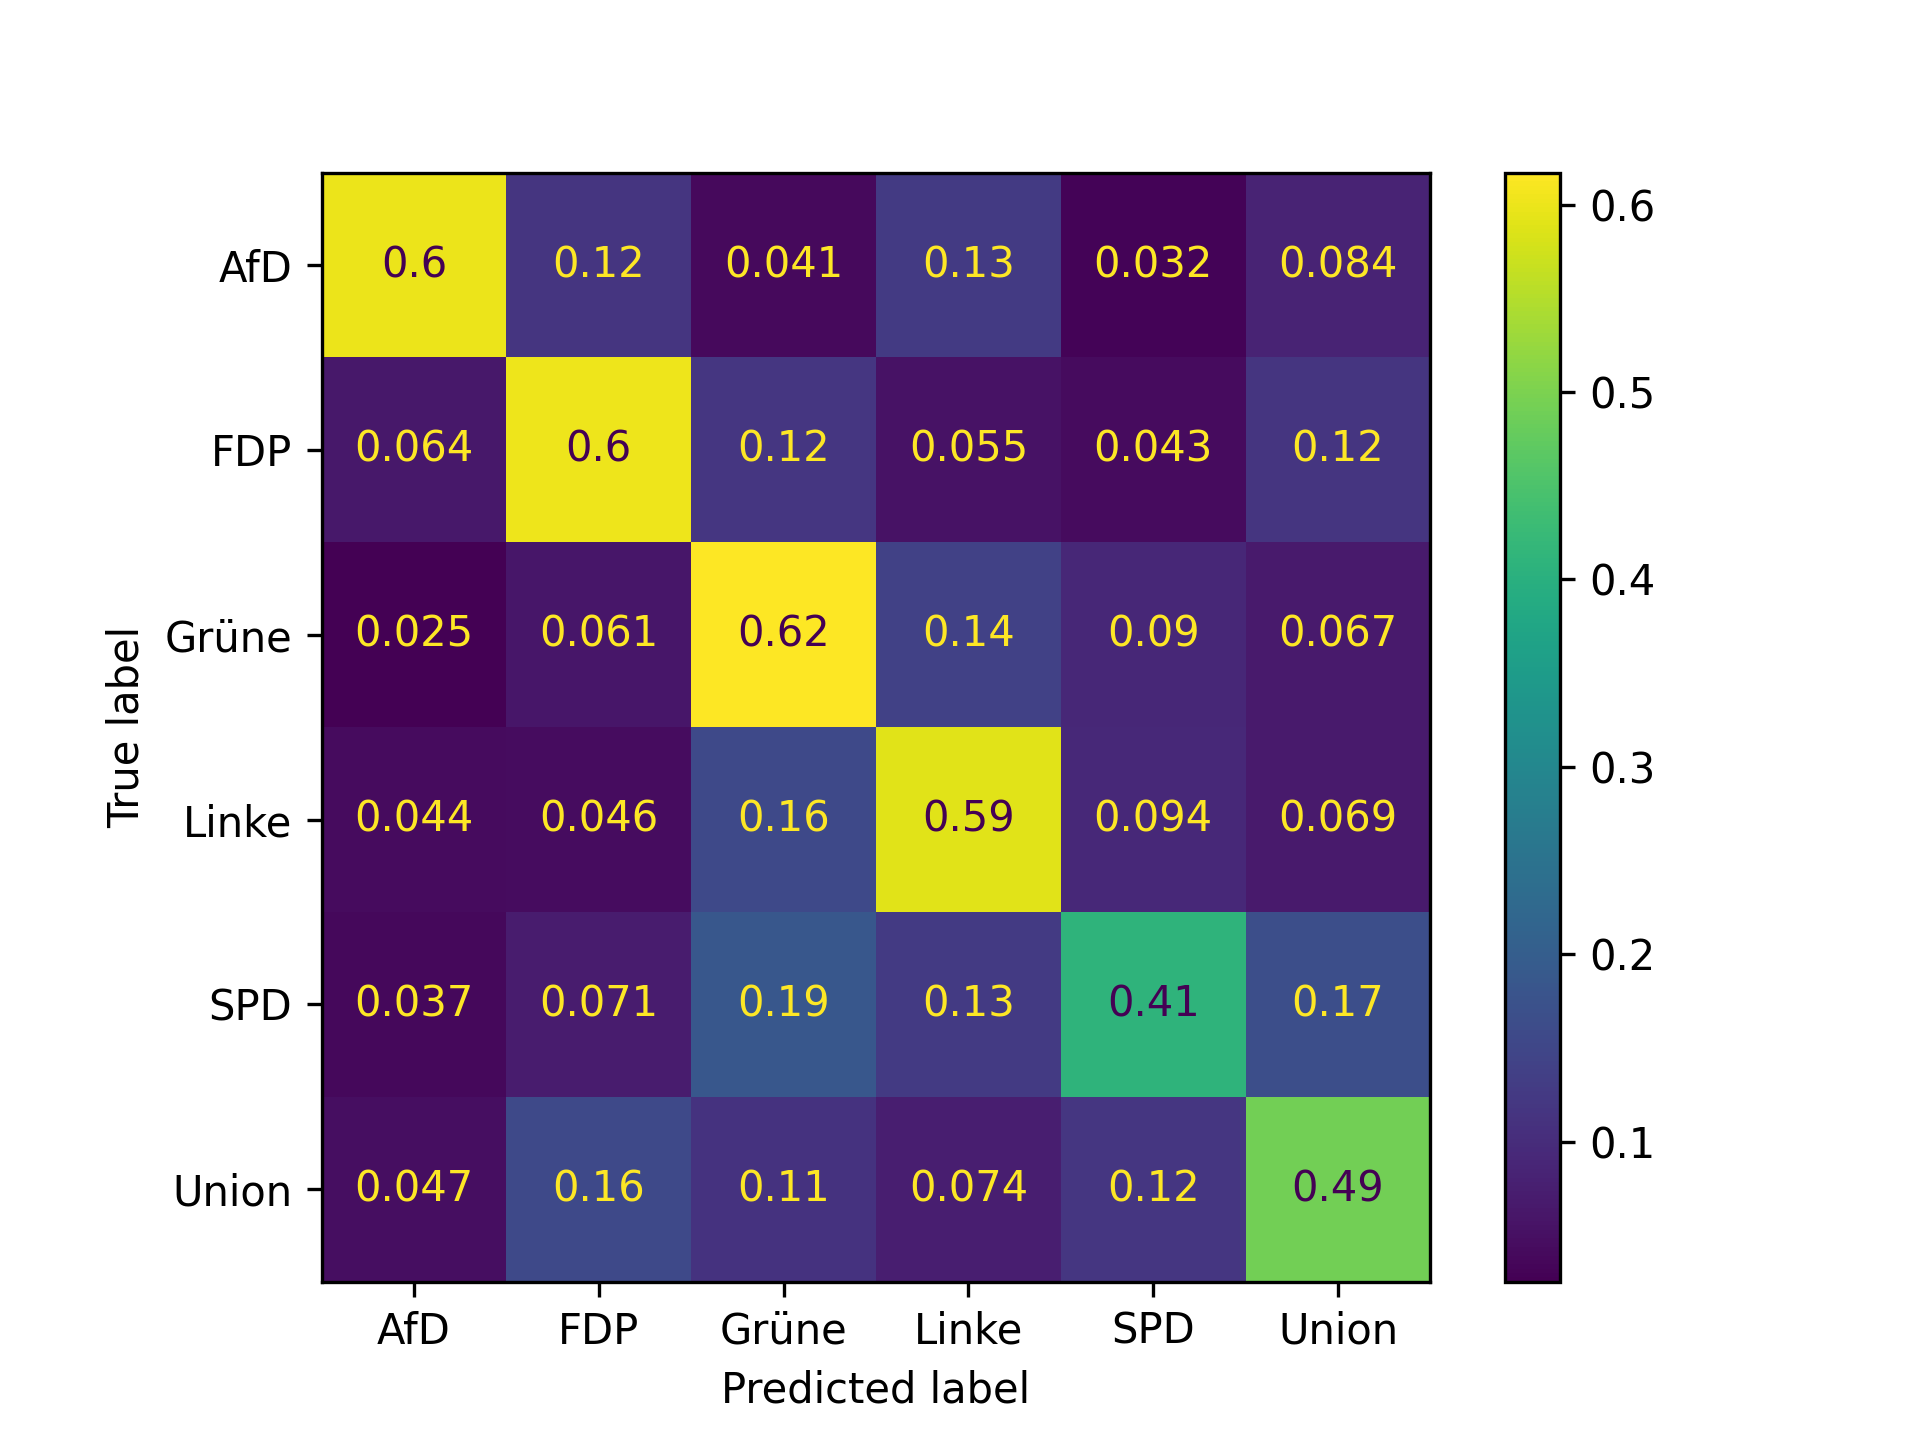
\includegraphics[width=\textwidth]{data/images/modeling/baseline/party_programs_confusion_matrix.png}
        \caption{Wahlprogramme (\(N=\num{27674}\))}
        \label{sfig:confusionMatrixBaselineManifest}
    \end{subfigure}
    \hfill
    \begin{subfigure}{0.49\textwidth}
        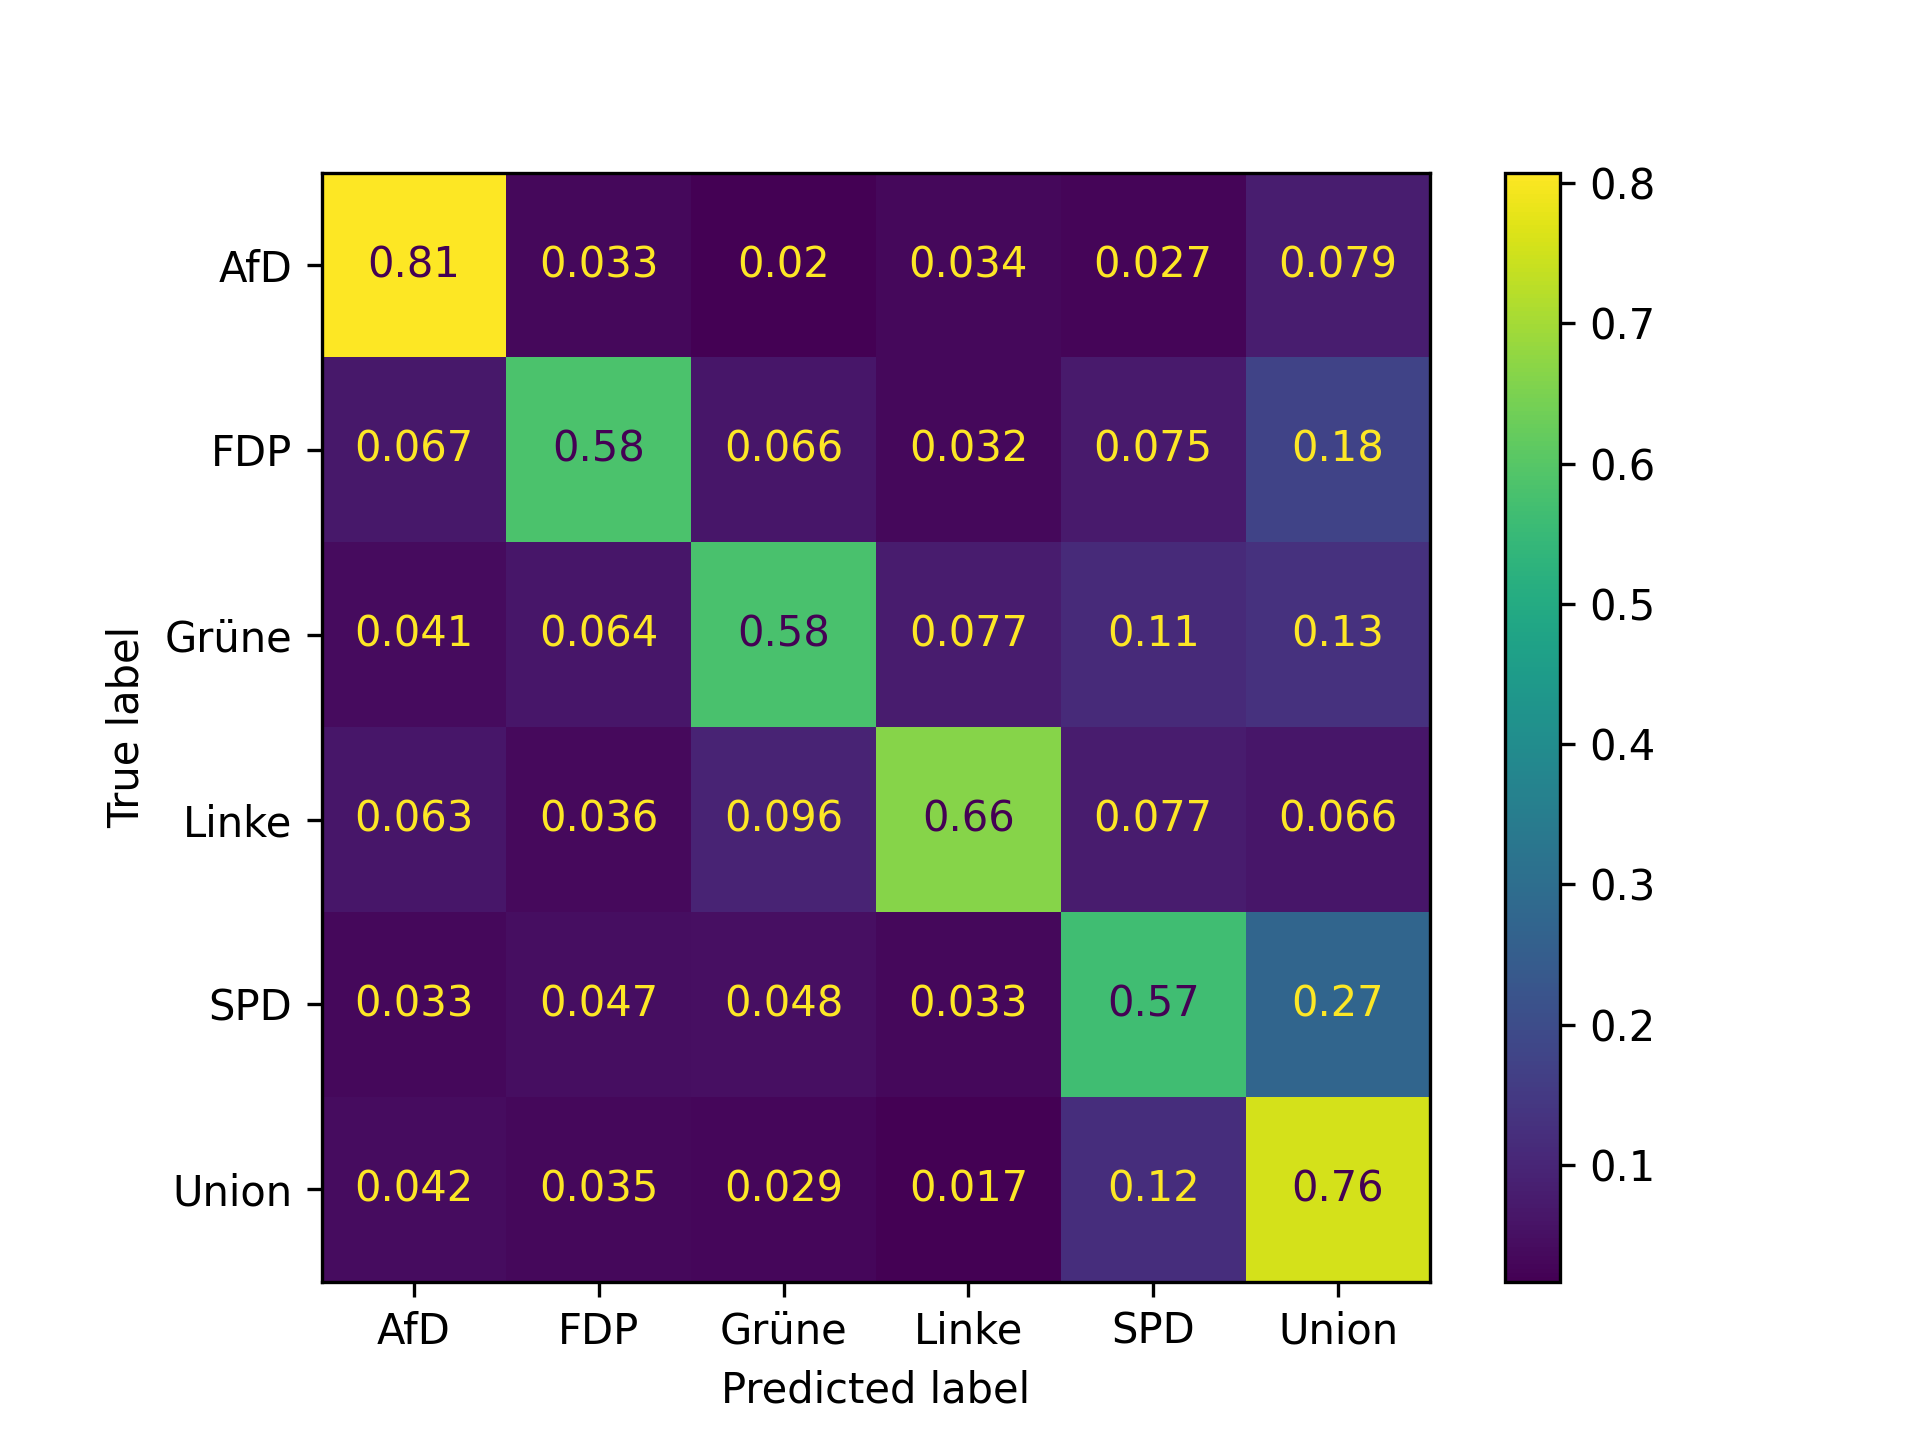
\includegraphics[width=\textwidth]{data/images/modeling/baseline/speeches_confusion_matrix.png}
        \caption{Reden (\(N=\num{38475}\))}
        \label{sfig:confusionMatrixBaselineSpeeches}
    \end{subfigure}
    \caption[Konfusionsmatrizen für Lineare \acs{SVC} mit \acs{TF-IDF} auf unausgeglichenen Datensätzen]{Konfusionsmatrizen für Lineare \acs{SVC} und \acs{TF-IDF} auf unausgeglichenen Datensätzen. $N$ repräsentiert die Anzahl an Trainings- und Testdaten.} \label{fig:confusionMatrixBaseline}
\end{figure}

Bei den Tweets (\autoref{sfig:confusionMatrixBaselineTweets}) lässt sich die \ac{AfD} am besten klassifizieren. Unter allen Tweets, die als \ac{AfD} klassifiziert wurden, stimmen \SI{65}{\percent} überein. Die Matrix zeigt keine Partei, welche häufig mit der \ac{AfD} verwechselt wurde. Am zweitbesten, mit \SI{58}{\percent}, erkennt das Modell Tweets der Linken. Am häufigsten wird die Linke mit den anderen beiden Parteien im linken Spektrum verwechselt (True-Negative). Somit werden zu \SI{13}{\percent} Tweets der Linken den Grünen und \SI{11}{\percent} der \ac{SPD} zugeordnet. Dasselbe Phänomen tritt bei den Tweets der Grünen auf. Bei den Tweets der \ac{SPD} kommt zu Grünen und Linken die Union hinzu. Die Tweets der Union selbst werden zu \SI{15}{\percent} als \ac{SPD} klassifiziert. Tweets der \ac{FDP} werden zu jeweils \SI{12}{\percent} den Grünen und der Union zugeordnet. Allgemein ist festzuhalten, dass Tweets einer politischen Partei häufig als politisch nahestehende Partei klassifiziert werden. Weiterhin ist festzustellen, dass die False-Negative und True-Negativ Raten in \autoref{sfig:confusionMatrixBaselineTweets} symmetrisch entlang True-Positive Achse auftreten.

Die \autoref{sfig:confusionMatrixBaselineManifest} zeigt die Konfusionsmatrix für die Wahlprogramme. Parteien, die eine politische Nähe aufweisen, weisen ebenfalls wie bei den Tweets eine höhere True-Negative Rate. Auffällig ist, dass die True-Positive Rate bei \ac{SPD} und der Union deutlich schlechter ist als bei den anderen Parteien. Die beiden Regierungsparteien erreichen \SIrange{41}{49}{\percent}, während die Oppositionsparteien \SIrange{59}{62}{\percent} erreichen. Dies zeigt sich ebenfalls in der True-Negative Rate der beiden Parteien. Abweichend von den Tweets, weist die \ac{AfD} eine hohe True-Negative Rate bei der \ac{FDP} und der Linken auf.

Der Datensatz der Reden führt insgesamt zu der höchsten Genauigkeit. Die Konfusionsmatrix \autoref{sfig:confusionMatrixBaselineSpeeches} zeigt, dass die Reden der \ac{AfD} mit \SI{81}{\percent} und der Union mit \SI{76}{\percent} am besten klassifiziert werden. Die Reden der anderen Parteien erreichen für die True-Positive Rate lediglich zwischen \SIrange{57}{66}{\percent}. Grundsätzlich weist die Konfusionsmatrix für die Reden wenige Übereinstimmungen mit den anderen beiden Matrizen im allgemeinen Muster auf. Im Gegensatz zu den Tweets und Wahlprogrammen werden die Reden der Grünen auffallend oft als Reden der \ac{SPD} oder der Union klassifiziert. Die stärkste Verwechslung für True-Negativ über alle Datensätze hinweg tritt bei Reden der \ac{SPD} auf. Diese werden zu \SI{27}{\percent} als Reden der Union klassifiziert. Die Reden der Union werden ebenfalls zu \SI{12}{\percent} der \ac{SPD} zugeordnet. 

Bei allen drei Konfusionsmatrizen weisen die \ac{SPD} und \ac{CDU} eine starke gegenseitige Verwechselung auf. Ein weiterer Faktor, neben der politischen Nähe, könnte sein, dass die beiden Parteien im Untersuchungszeitraum zusammen die Regierung gebildet haben.

\subsection{fastText}

\ft ist eine Methode zum Generieren von Worteinbettungen, die von Facebook Research entwickelt wird \autocite{joulin_bag_2016}. Wie schon in \autoref{sec:representationForms} dargelegt, basiert die Methodik darauf, Wörter in n-grams zu zerlegen. Resultierend lassen sich ebenfalls Wörter klassifizieren, welche nicht im Trainingsdatensatz für die Worteinbettungen enthalten waren \autocite{guhr_training_2020}. Auf den sich ergebenden Worteinbettungen kann schließlich ein Klassifikator trainiert werden.

Für das folgende Training wird die \href{https://pypi.org/project/fasttext/}{\ft} Bibliothek für Python verwendet. Um die Worteinbettungen von \ft zu nutzen ist es möglich entweder eigenständig die Einbettungen zu trainieren oder vortrainierte Einbettungen zu verwenden. Im Rahmen dieser Arbeit werden \href{https://fasttext.cc/docs/en/crawl-vectors.html}{vortrainierte Einbettungen} verwendet, da die eigene Erstellung solcher Einbettungen eine große Menge an Daten benötigt. Die vortrainierten, deutschen Worteinbettungen basieren auf dem \href{https://commoncrawl.org/}{Common Crawl} und \href{https://www.wikipedia.org/}{Wikipedia} Datensatz.

Für das Training werden die Hyperparameter von \textcite{guhr_training_2020} übernommen. Demnach wird mit allen Einträgen pro Datensatz für \num{20} Epochen und einer Lernrate von \num{0.1} trainiert. Für das Training werden ebenfalls Bigramme verwendet. Zusätzlich zu \citeauthor{guhr_training_2020} werden Trigramme verwendet. Im Gegensatz zu \textcite{guhr_training_2020} werden, die zuvor beschriebenen, vortrainierte Worteinbettungen mit einer Vektorgröße von \num{300} verwendet.

{\footnotesize
\begin{longtblr}[caption={Makro \(F_1\) Score für \ft}, label={tab:overviewScoresFastText}, remark{Parameter} = {\(E = \num{20}\), \(LR = \num{0.1}\)}]{hline{1, 3, Z} = {1pt}, rowhead = 2, colspec={l*{4}{Q[si={table-format=1.2},c]}}, row{1-2}={guard,font=\bfseries,l}}
     & \SetCell[c=2]{c} Bigramme (\(n = \num{2}\)) & & \SetCell[c=2]{c} Trigramme (\(n = \num{3}\)) & \\ 
    \cline{2-5}
    Datensatz & Unbalanced & Balanced & Unbalanced & Balanced \\ 

    Tweets & \textbf{\num{0.59}} & 0.58 & \textbf{\num{0.59}} & 0.57 \\*
    Wahlprogramm & \textbf{\num{0.58}} & 0.54 & 0.57 & 0.54 \\*
    Reden & \textbf{\num{0.69}} & 0.65 & 0.67 & 0.66 \\*
    \hline
    Kombiniert & \textbf{\num{0.59}} & 0.57 & 0.58 & 0.57 \\
\end{longtblr}
}

\autoref{tab:overviewScoresFastText} zeigt, die Makro \(F_1\) Scores, die mittels \ft erreicht wurden. Das Training erfolgte auf Bi- und Trigrammen. Aus den Ergebnissen geht hervor, dass durchweg das Training auf den unbalancierten Datensätzen zu höheren \(F_{1}\) Scores geführt hat. Auf den unbalancierten Daten mit Bigrammen erreichen Tweets und Wahlprogramme einen \(F_{1}\) von \numrange{0.58}{0.59}. Den höchsten Wert erreichen die Reden mit \num{0.69}. Auf den balancierten Daten schneiden die Bigramme zwischen \numrange{0.01}{0.04} schlechter ab. Lediglich auf den unbalancierten Tweets erreichen Trigrammen den identischen Score wie auf Bigrammen. Die unbalancierten Wahlprogramme und Reden schneiden jeweils \num{0.02} schlechter ab. Auf den balancierten Wahlprogrammen erreichen Trigramme ebenfalls den gleichen Wert, während Tweets und Reden jeweils um \num{0.01} schlechter abschneiden.

Auf den kombinierten, unbalancierten Daten erreichen die Bigramme einen Makro \(F_1\) Score von \num{0.59}. Den zweitbesten Wert erreichen die Trigramme ebenfalls auf unbalancierten Daten. Auf balancierten Daten erreichen Bi- und Trigramme einen Wert von \num{0.57}.

% TODO: Alle Parameter beschreiben

\begin{figure}[H]
    \centering
    \begin{subfigure}{0.49\textwidth}
      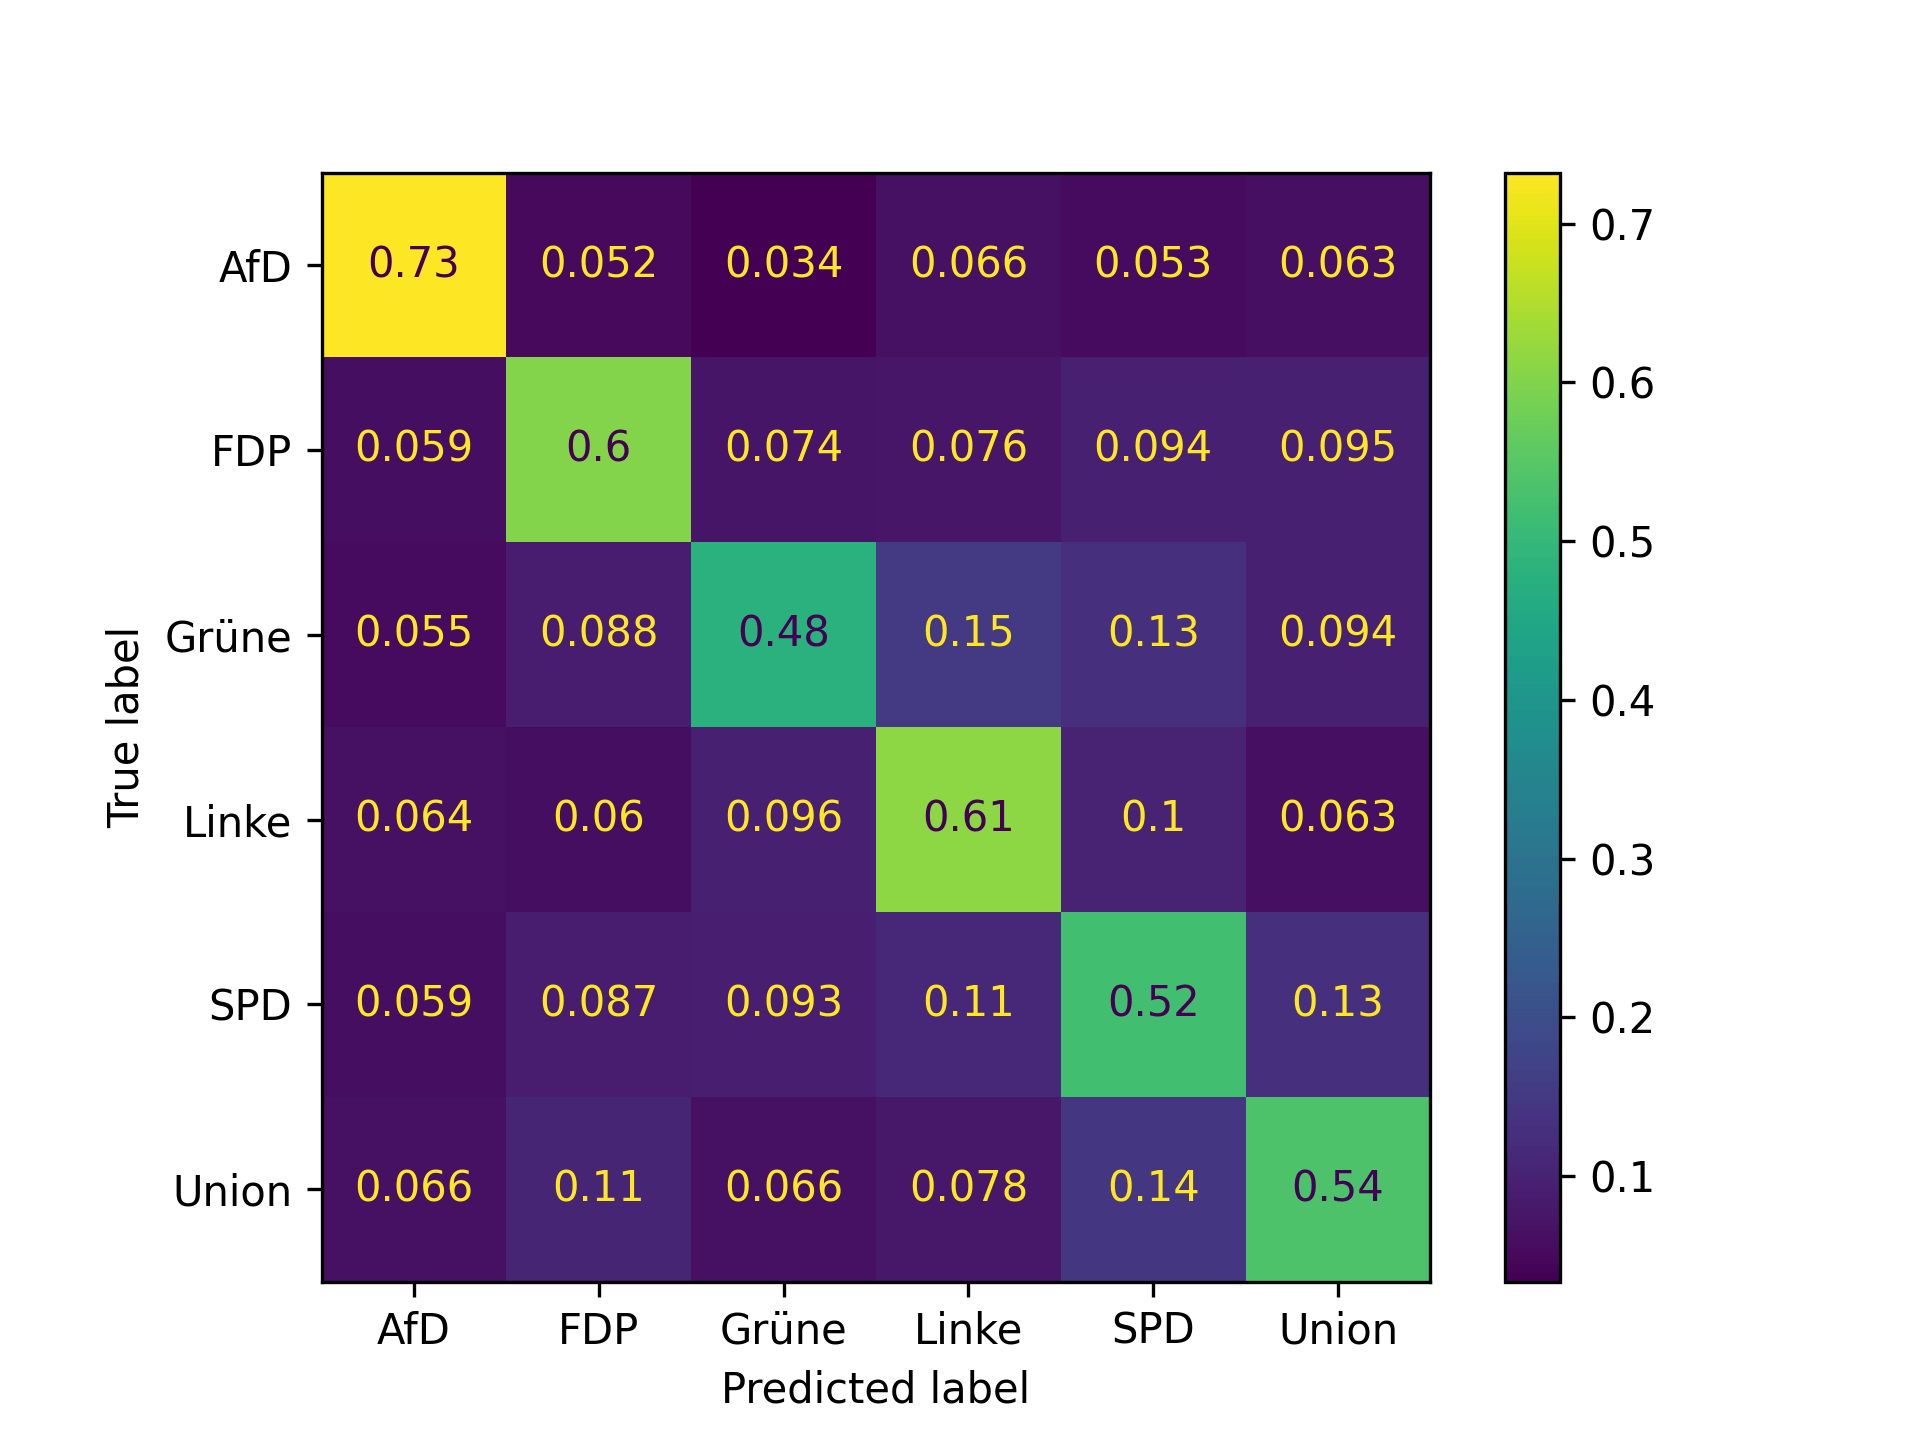
\includegraphics[width=\textwidth]{data/images/modeling/fasttext/under/tweets_confusion_matrix.png}
      \caption{Tweets (\(N = \num{255813}\))} \label{sfig:confusionMatrixFastTextTweetsBalanced}
    \end{subfigure}
    \hfill
    \begin{subfigure}{0.49\textwidth}
      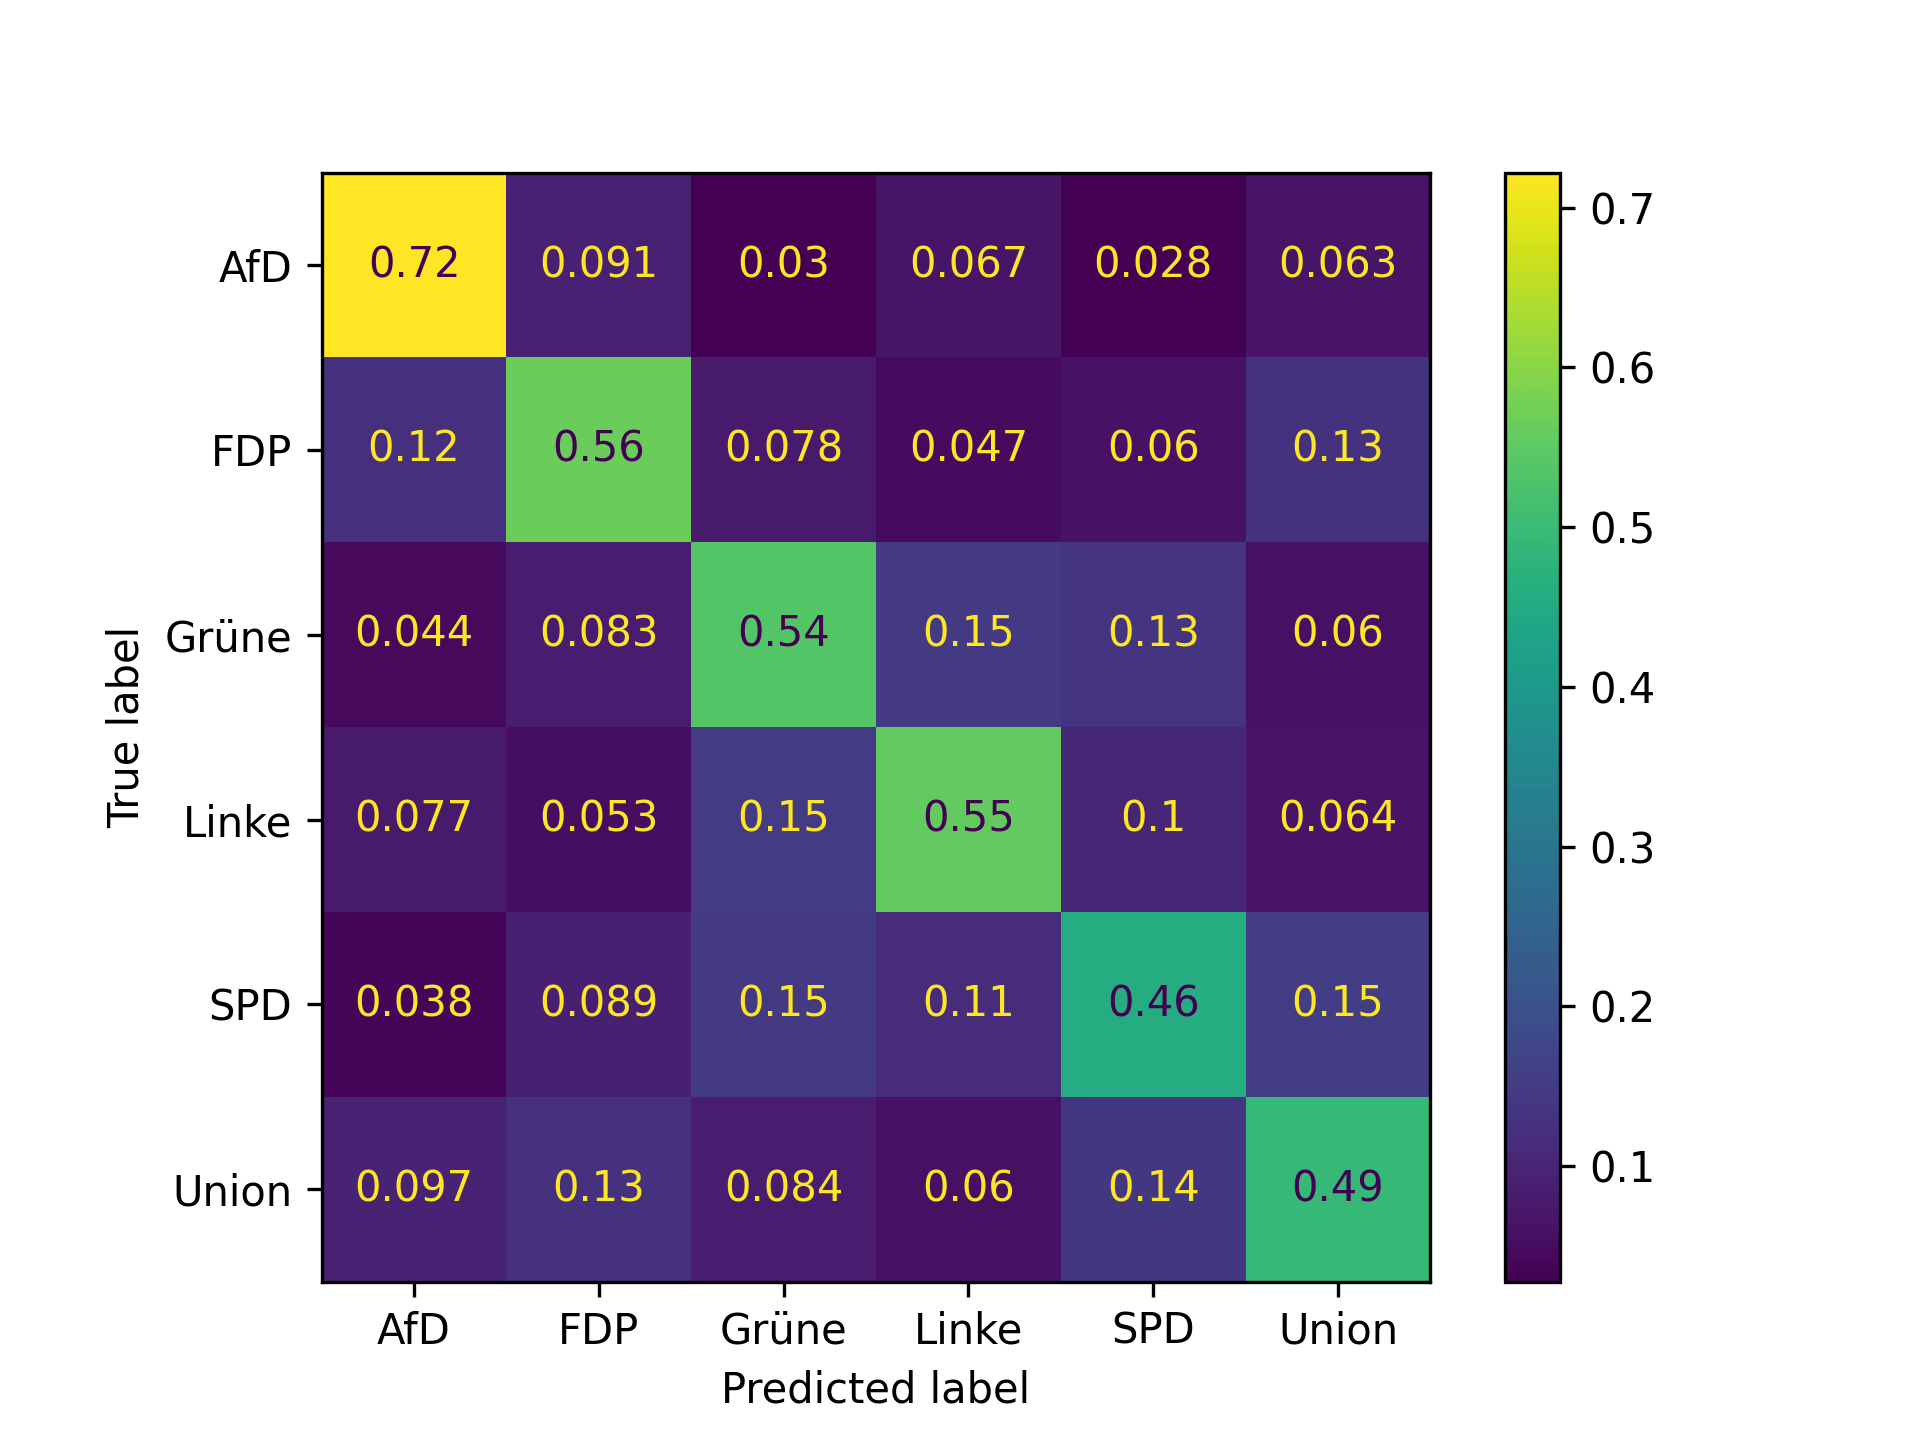
\includegraphics[width=\textwidth]{data/images/modeling/fasttext/under/party_programs_confusion_matrix.png}
      \caption{Wahlprogramme (\(N = \num{17949}\))} \label{sfig:confusionMatrixFastTextManifestBalanced}
    \end{subfigure}
    \hfill
    \begin{subfigure}{0.49\textwidth}
      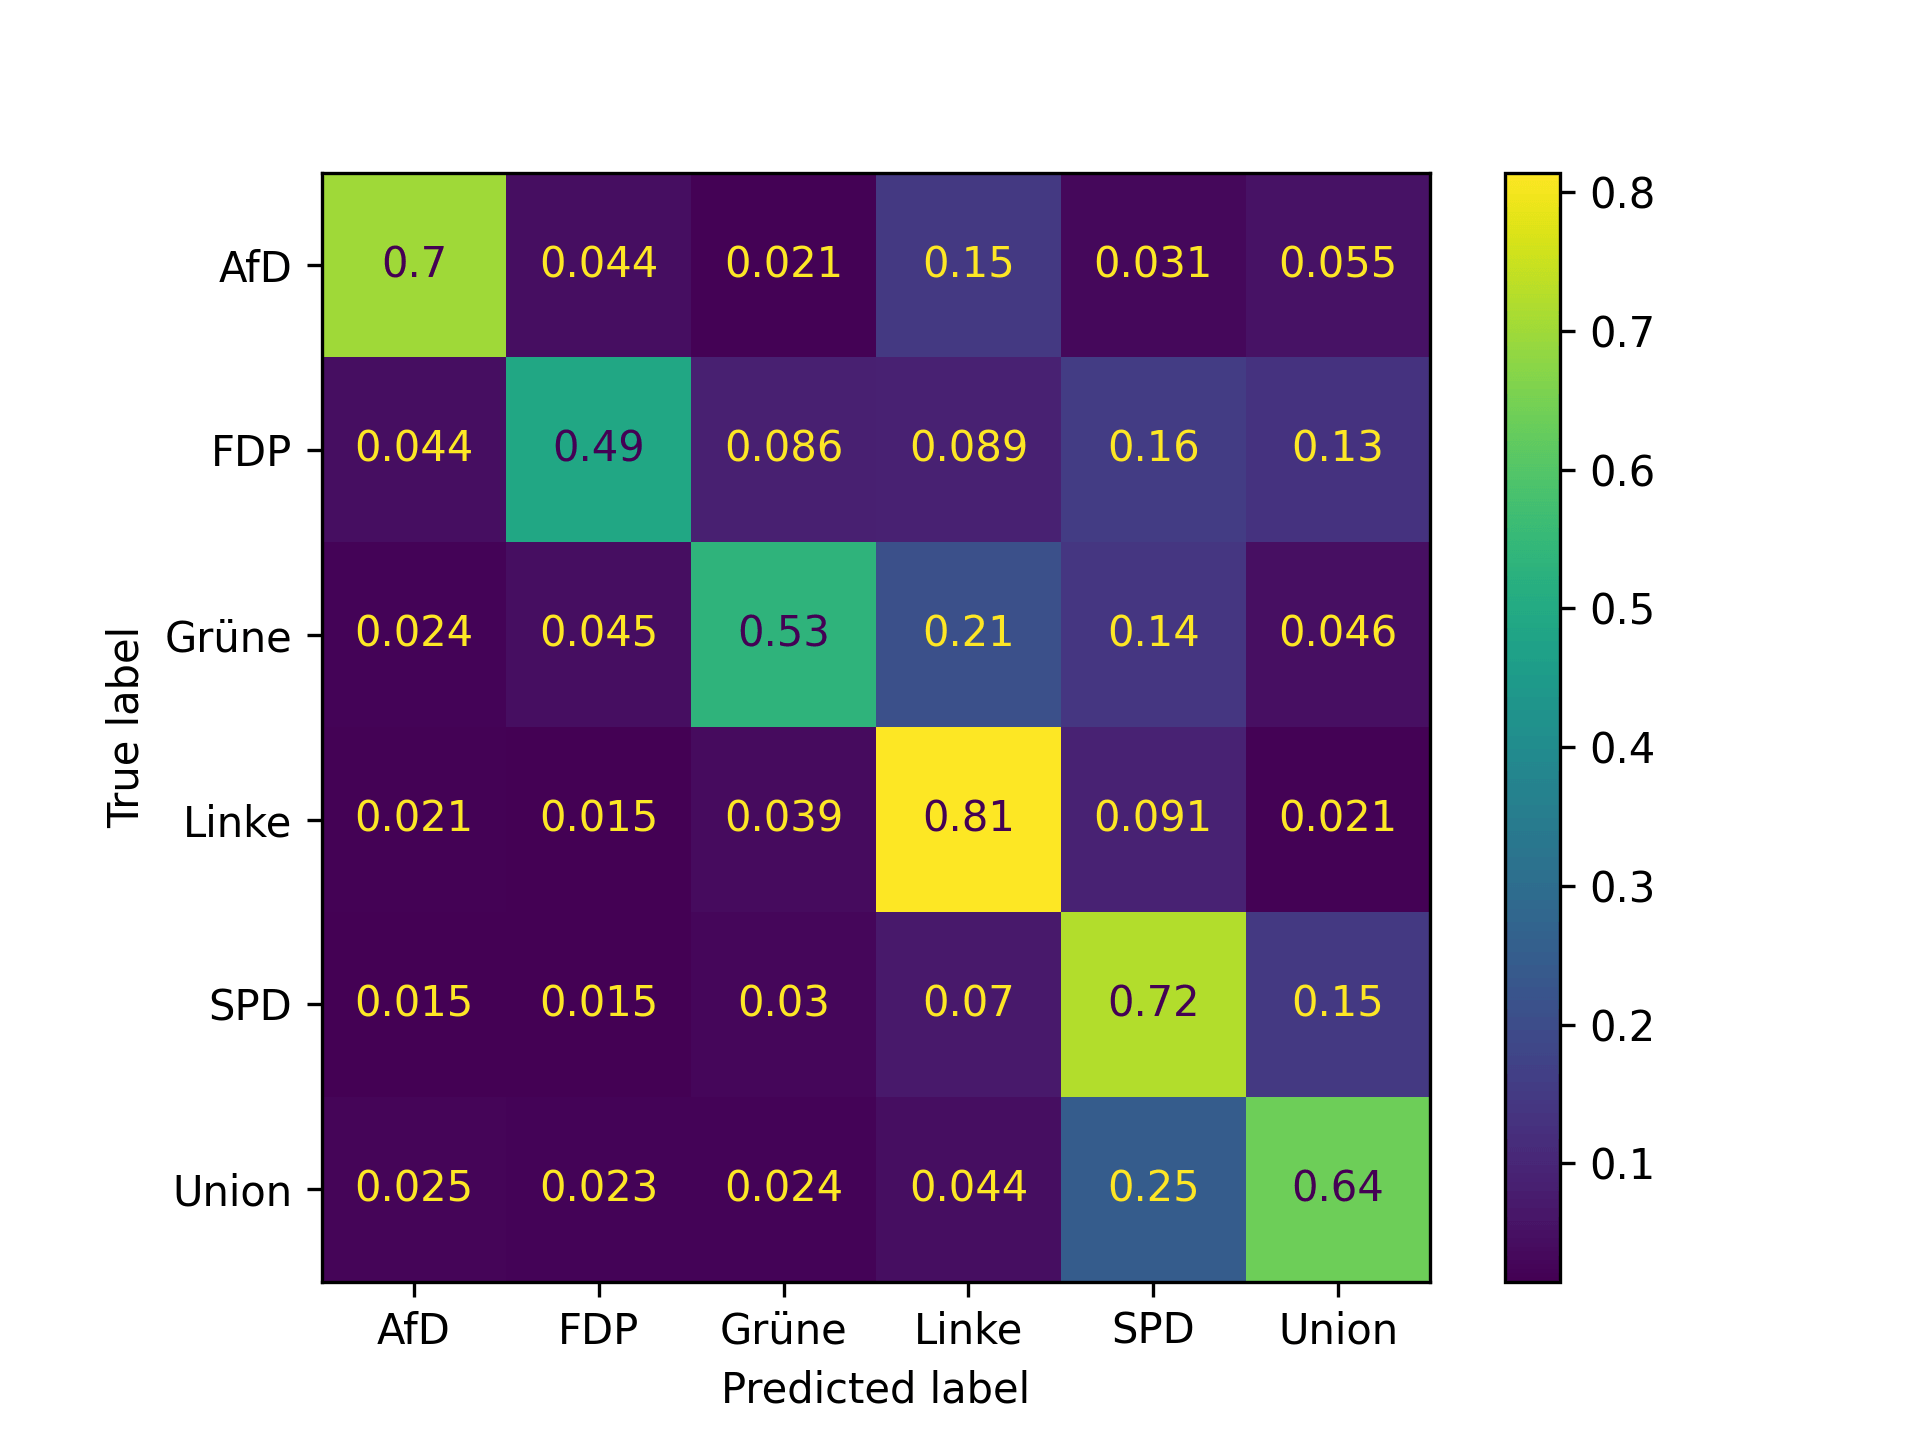
\includegraphics[width=\textwidth]{data/images/modeling/fasttext/under/speeches_confusion_matrix.png}
      \caption{Reden (\(N = \num{28719}\))} \label{sfig:confusionMatrixFastTextSpeechesBalanced}
    \end{subfigure}
    \hfill
    \begin{subfigure}{0.49\textwidth}
      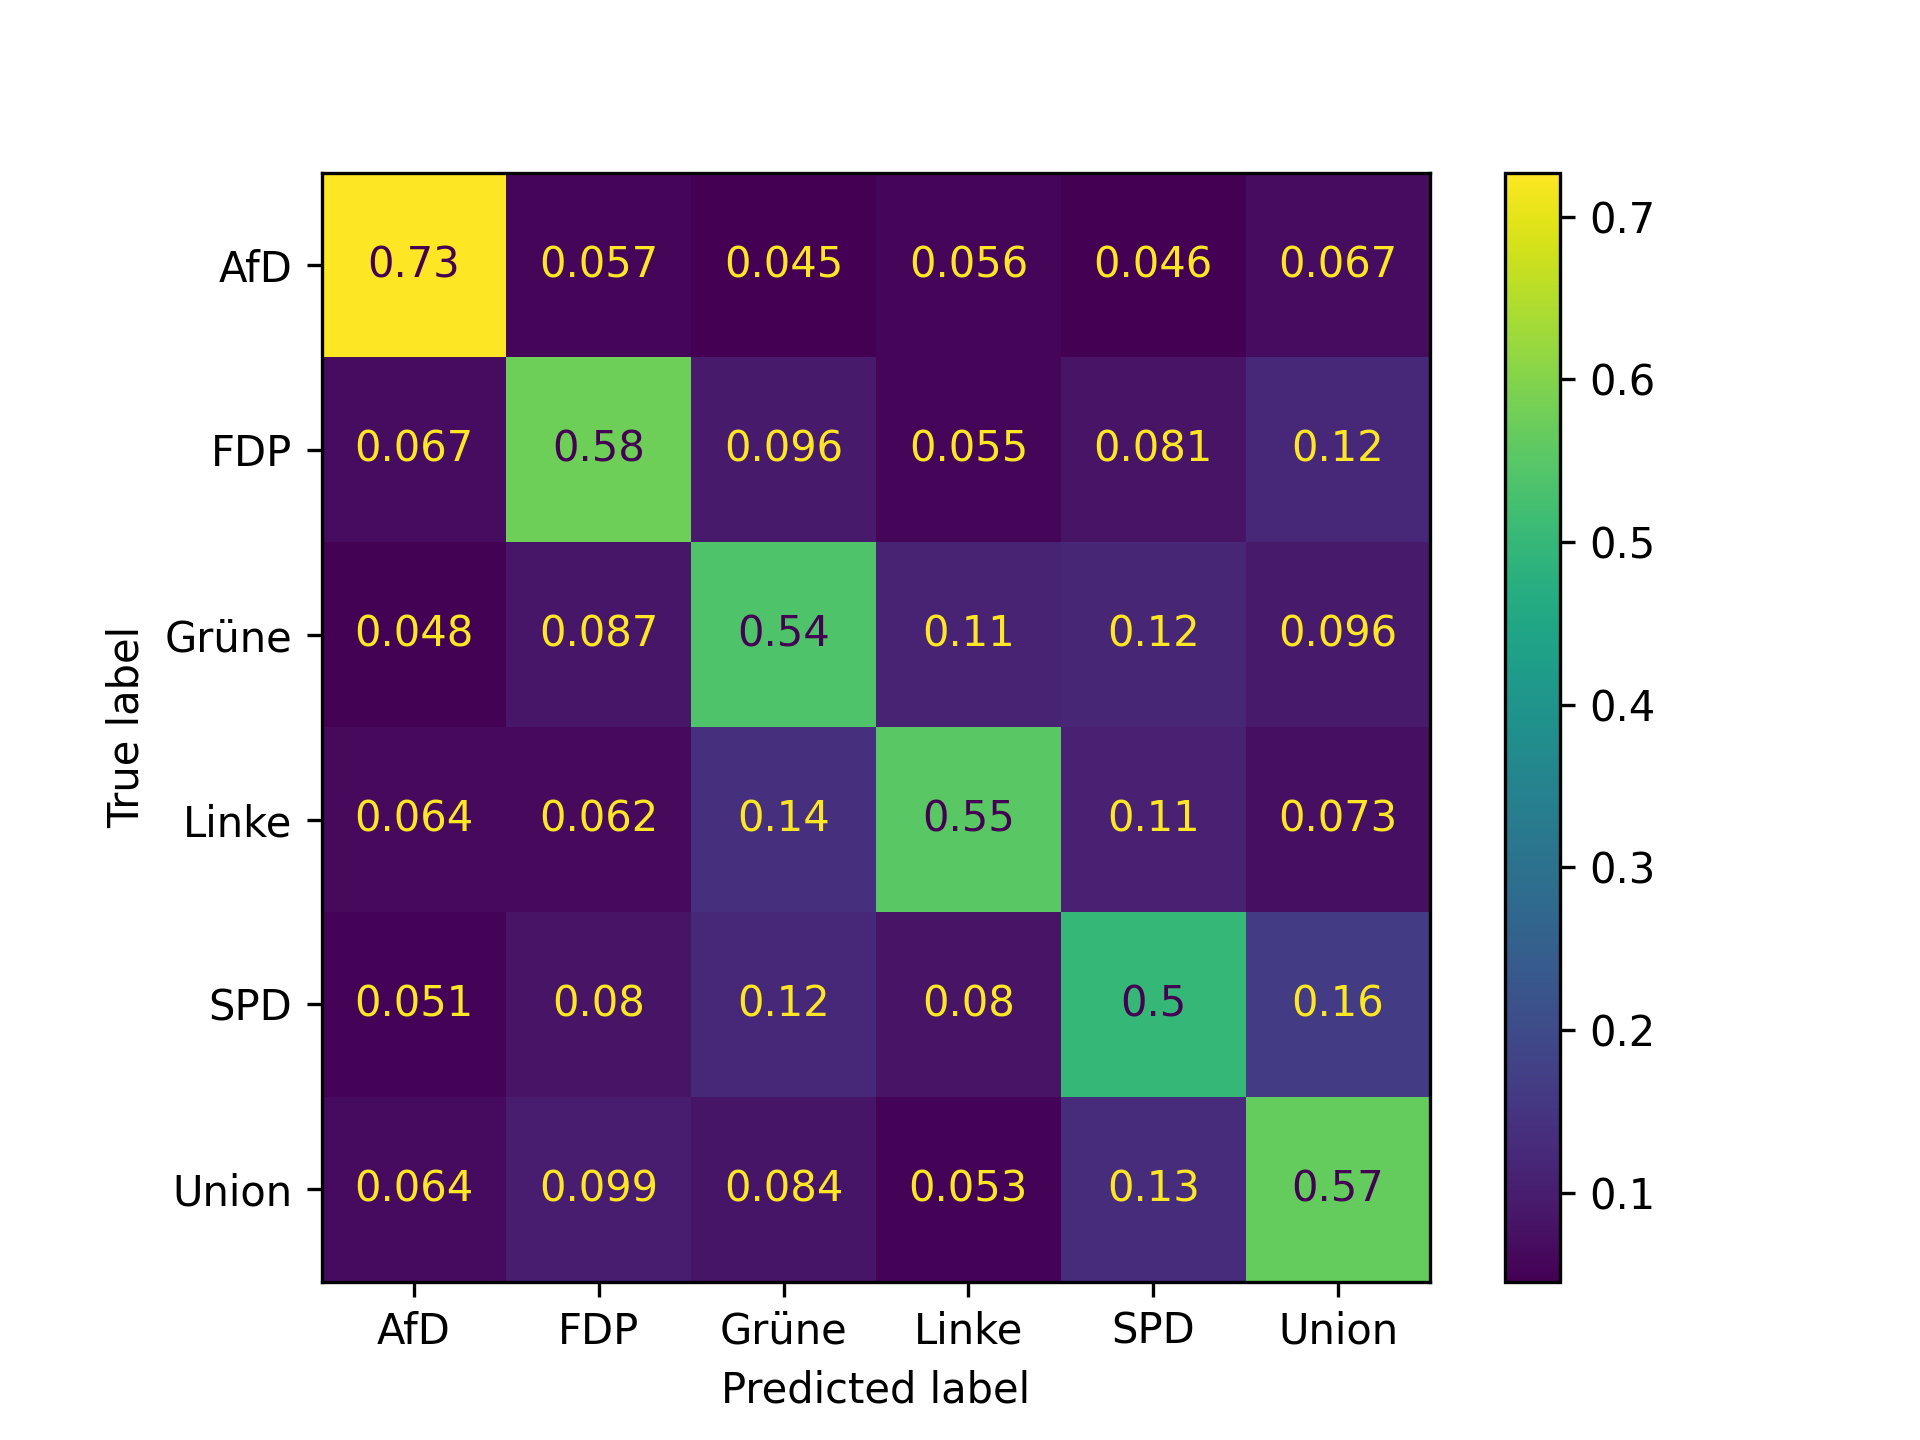
\includegraphics[width=\textwidth]{data/images/modeling/fasttext/under/all_confusion_matrix.png}
      \caption{Kombiniert (\(N = \num{308979}\))} \label{sfig:confusionMatrixFastTextAllBalanced}
    \end{subfigure}
    \caption[Konfusionsmatrizen für \ft mit Bigrammen (\(n = \num{2}\)) auf ausgeglichenen Datensätzen]{Konfusionsmatrizen für \ft mit Bigrammen (\(n = \num{2}\)) auf ausgeglichenen Datensätzen. \(N\) repräsentiert die summierte Anzahl an Trainings- und Testdaten.} \label{fig:balancedConfusionMatrixFastText}
\end{figure}

% Bei Tweets -> durchmischt
% Wahlprogramme -> links rechts
% Reden -> Politische nähe sealtzer

\begin{itemize}
    \item Parteien, die politisch näher beieinander liegen, lassen sich schlechter klassifizieren
    \item \ft ist sehr anfällig für unbalancierte Datensätze
    \item Regierungsparteien neigen zu hoher True Negative Rate untereinander
    \item True Negative Rate segmentiert sich nach Regierungsparteien und Opposition (besonders bei Reden)
\end{itemize}

\subsection{Multi-Layer Perceptron}

\sk bietet mit der Klasse \texttt{MLPClassifier} die einfache Möglichkeit, ein \ac{MLP} für die Klassifikation zu trainieren. Bei einem \ac{MLP} handelt es sich um ein simples neuronales Netzwerk mit einer Eingabeschicht, einer Ausgabeschicht und optionalen Zwischenschichten. Als Eingabedaten wird mittels \ac{BoW} oder \ac{TF-IDF} vektorisierter Text verwendet. Dafür gilt die gleiche Konfiguration wie bereits in \autoref{subsec:baseline} dargelegt sowie die Limitation auf \num{125000} Tweets aus Ressourcengründen.

Eine Hyperparameteroptimierung durch eine Rastersuche liefert als beste Architektur ein Netz mit einer Zwischenschicht bestehend aus \num{100} Neuronen (\(hidden\_layer\_sizes=(100,)\)) sowie der Verwendung der \ac{ReLU}-Aktivierungsfunktion (\(activation=relu\)). Die Lernrate wird initial auf \num{7e-4} gesetzt und nach jeder Iteration graduell verringert (\(learning\_rate=invscaling\)). Das Training in jeder Konfiguration läuft maximal \num{50} Iterationen lang (\(max\_iter=50\)).

{\footnotesize
\begin{longtblr}[caption={Macro \(F_1\) Score für \acs{MLP}-Modell}, label={tab:overviewScoresMlp}, note{$\dag$}={Aufgrund von beschränkten Rechenressourcen zum Training wird der Datensatz auf \num{125000} zufällig ausgewählte Einträge beschränkt.}, remark{Parameter MLP} = {\(activation=relu\), \(hidden\_layer\_sizes=(100,)\), \(learning\_rate=invscaling\), \(learning\_rate\_init=7e-4\), \(max\_iter=50\)}, remark{Parameter BoW \& TF-IDF} = {\(max\_df = \num{0.2}\), \(ngram\_range = (1, 1)\)}]{hline{1, 3, Z} = {1pt}, rowhead = 2, colspec={l*{4}{Q[si={table-format=1.2},c]}}, row{1-2}={guard,font=\bfseries,l}}
     & \SetCell[c=2]{c} BoW & & \SetCell[c=2]{c} TF-IDF & \\
    \cline{2-5}
    Datensatz & Unbalanced & Balanced & Unbalanced & Balanced \\

    Tweets\TblrNote{$\dag$} & \textbf{\num{0.50}} & \num{0.47} & \num{0.49} & \num{0.45} \\
    Wahlpro\-gramme & \num{0.52} & \num{0.51} & \textbf{\num{0.54}} & \num{0.51} \\
    Reden & \textbf{\num{0.66}} & \num{0.65} & \num{0.64} & \num{0.64} \\
\end{longtblr}
}

In \autoref{tab:overviewScoresMlp} ist der \(F_1\) Score für jede Trainingskombination mit dem \ac{MLP} dargestellt. Für den Tweet- (\num{0.50}) und den Reden-Datensatz (\num{0.66}) kommt die \ac{BoW}-gestützte Variante auf den höchsten Score; bei den Wahlprogrammen jene mit \ac{TF-IDF} (\num{0.54}). Es wird dabei jeweils der unbalancierte Datensatz verwendet. Für jede Repräsentationsform und sowohl auf dem unausgeglichenen als auch auf dem ausgeglichenen Datensätzen lässt sich mit den Wahlprogrammen ein besserer Wert erreichen als mit den Tweets, und mit den Reden ein besserer als mit den Wahlprogrammen. Das Ergebnis auf dem ausgeglichenen Datensatz liegt stets bis zu \num{0.03} unter dem des unausgeglichenen.

\begin{figure}[H]
\centering
\begin{subfigure}{0.49\textwidth}
    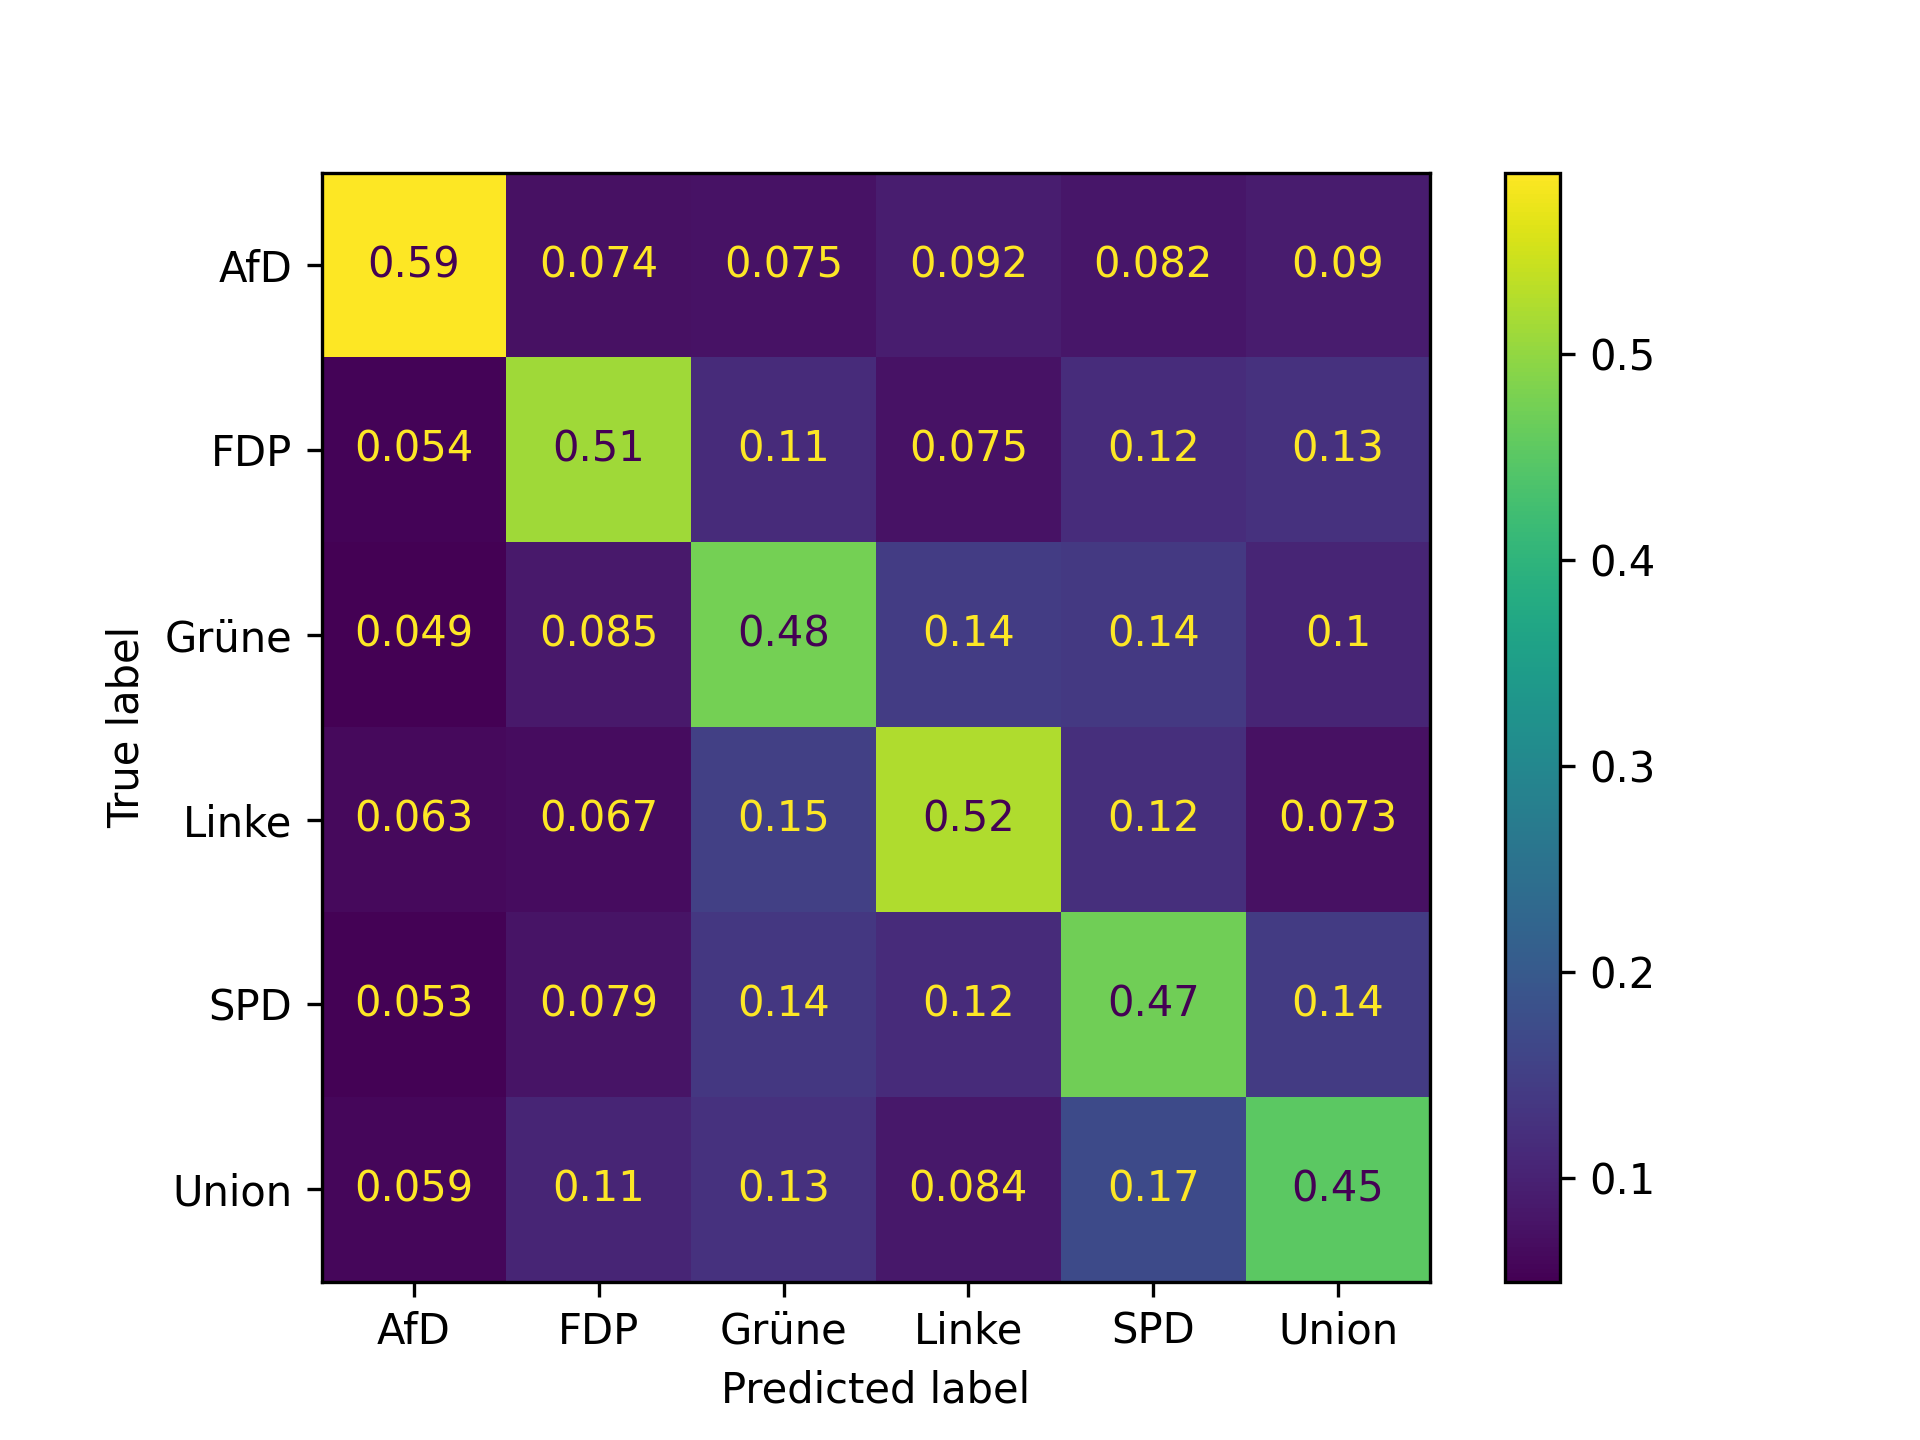
\includegraphics[width=\textwidth]{data/images/modeling/mlp/tweets_confusion_matrix.png}
    \caption{Tweets (\(N=\num{125000}\)), \ac{BoW}}
    \label{sfig:confusionMatrixMlpTweets}
\end{subfigure}
\hfill
\begin{subfigure}{0.49\textwidth}
    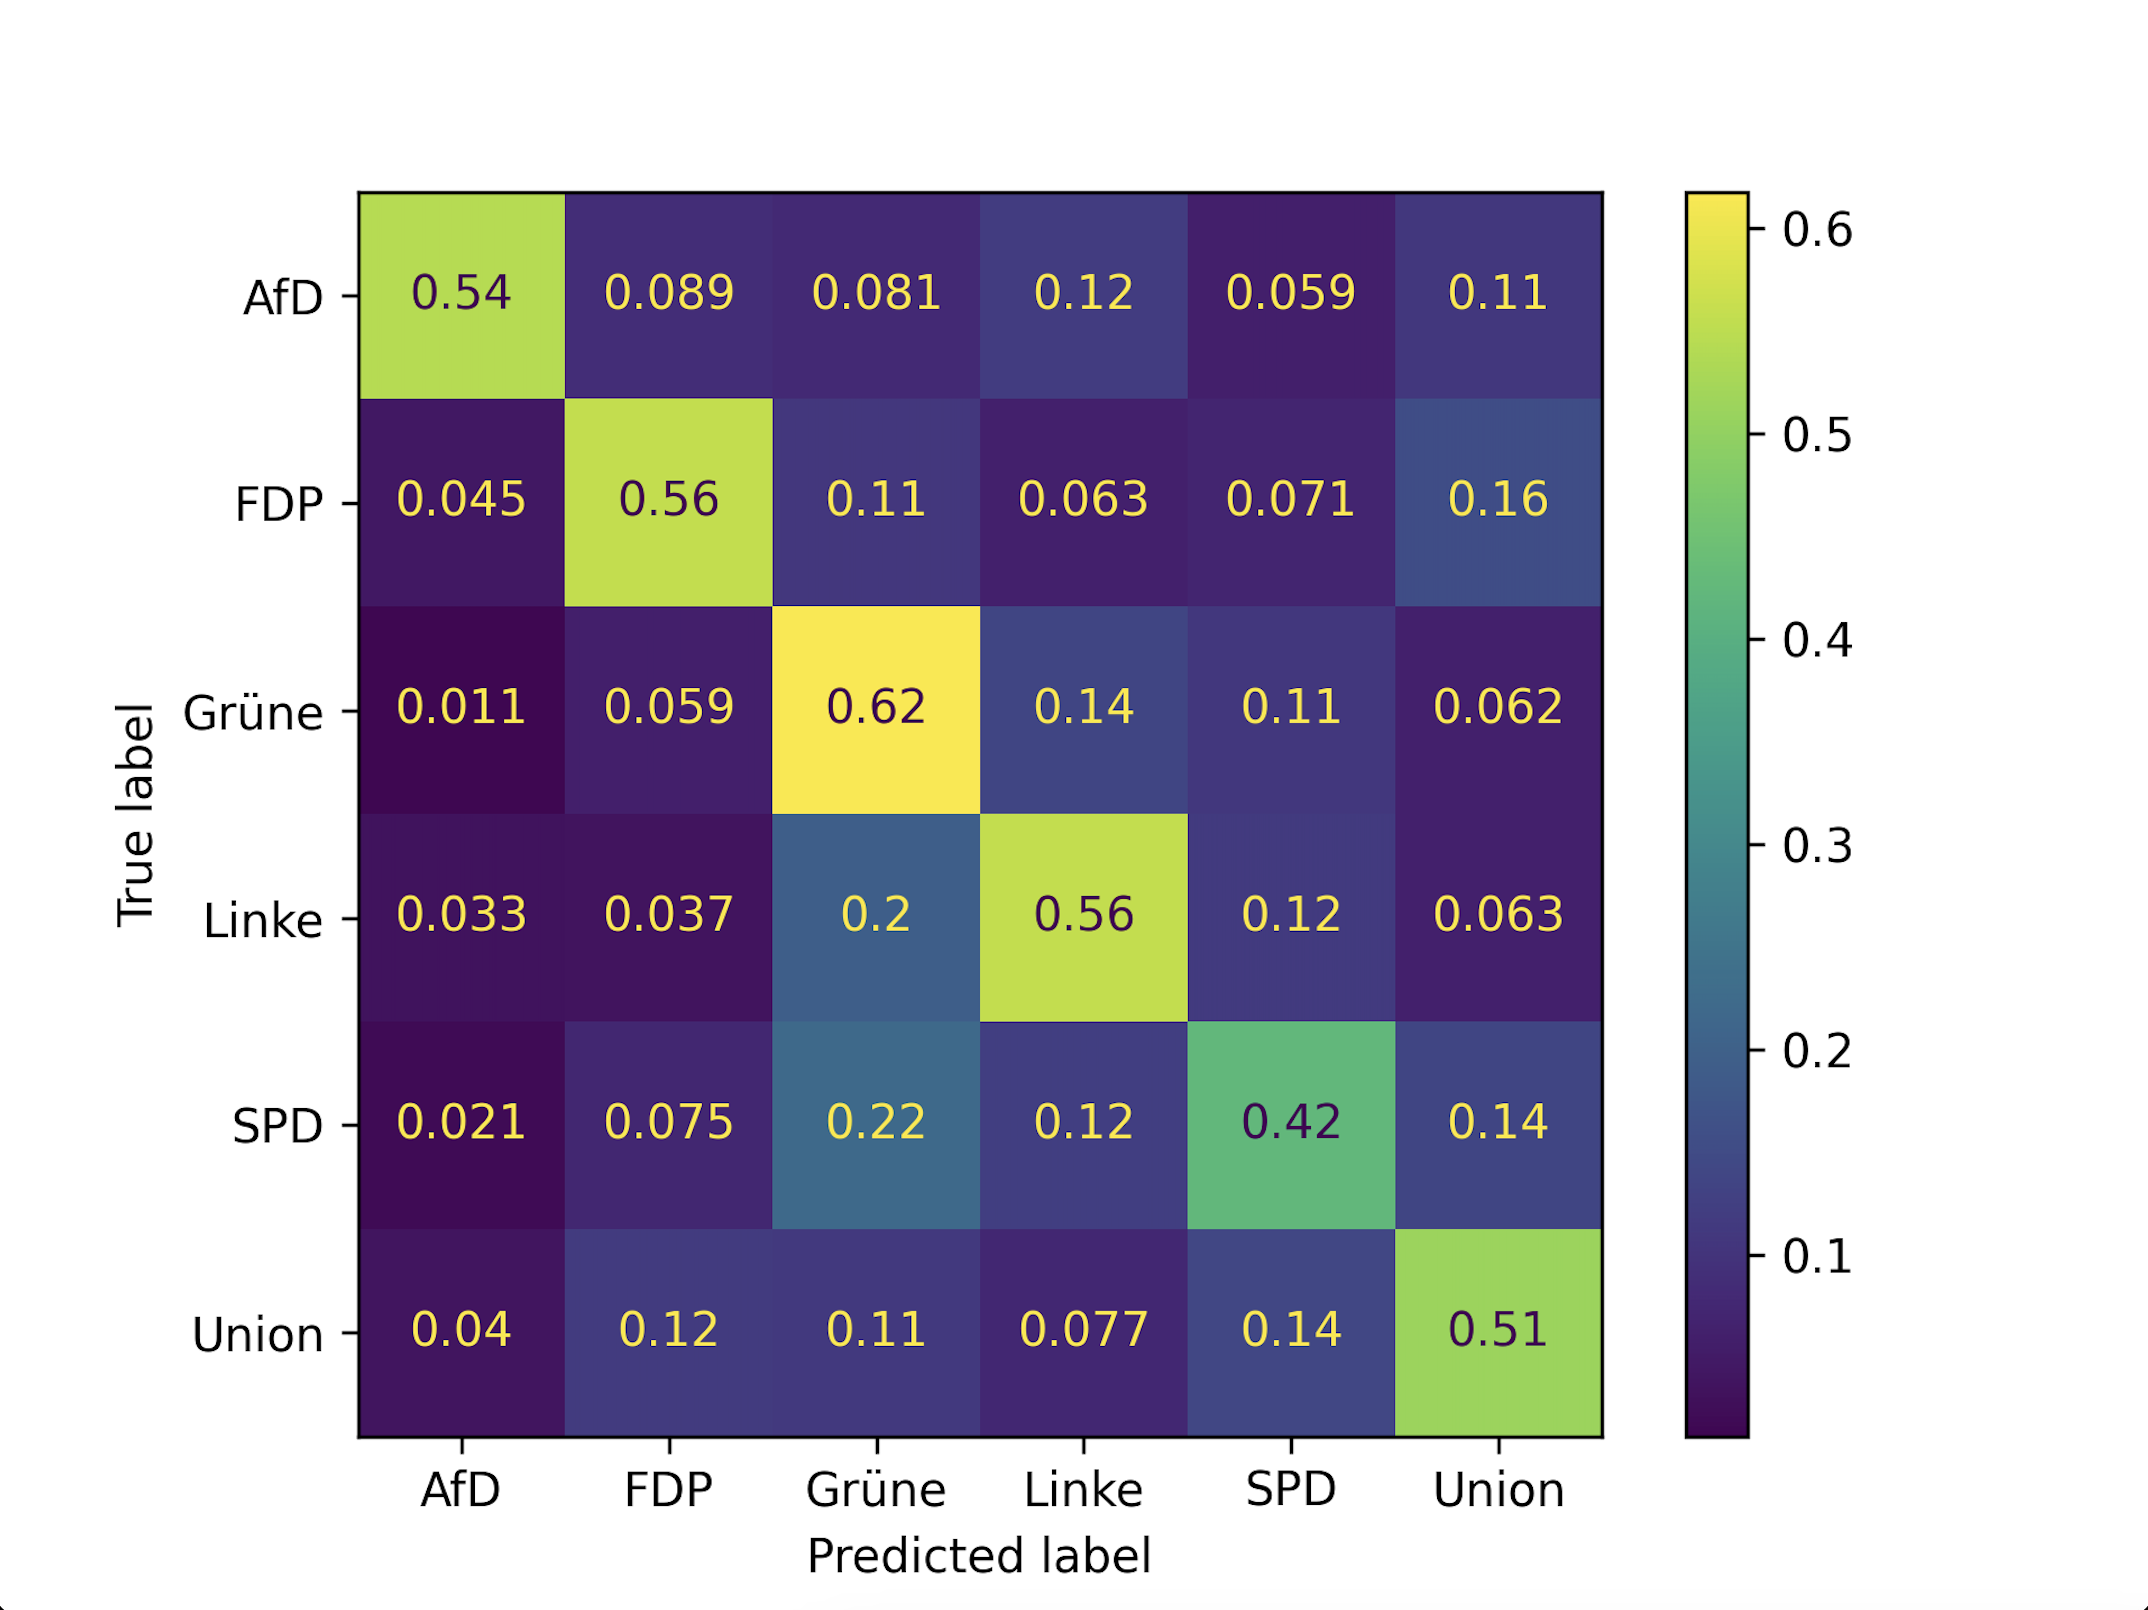
\includegraphics[width=\textwidth]{data/images/modeling/mlp/party_programs_confusion_matrix.png}
    \caption{Wahlprogramme (\(N=\num{27674}\)), \ac{TF-IDF}}
    \label{sfig:confusionMatrixMlpManifest}
\end{subfigure}
\hfill
\begin{subfigure}{0.49\textwidth}
    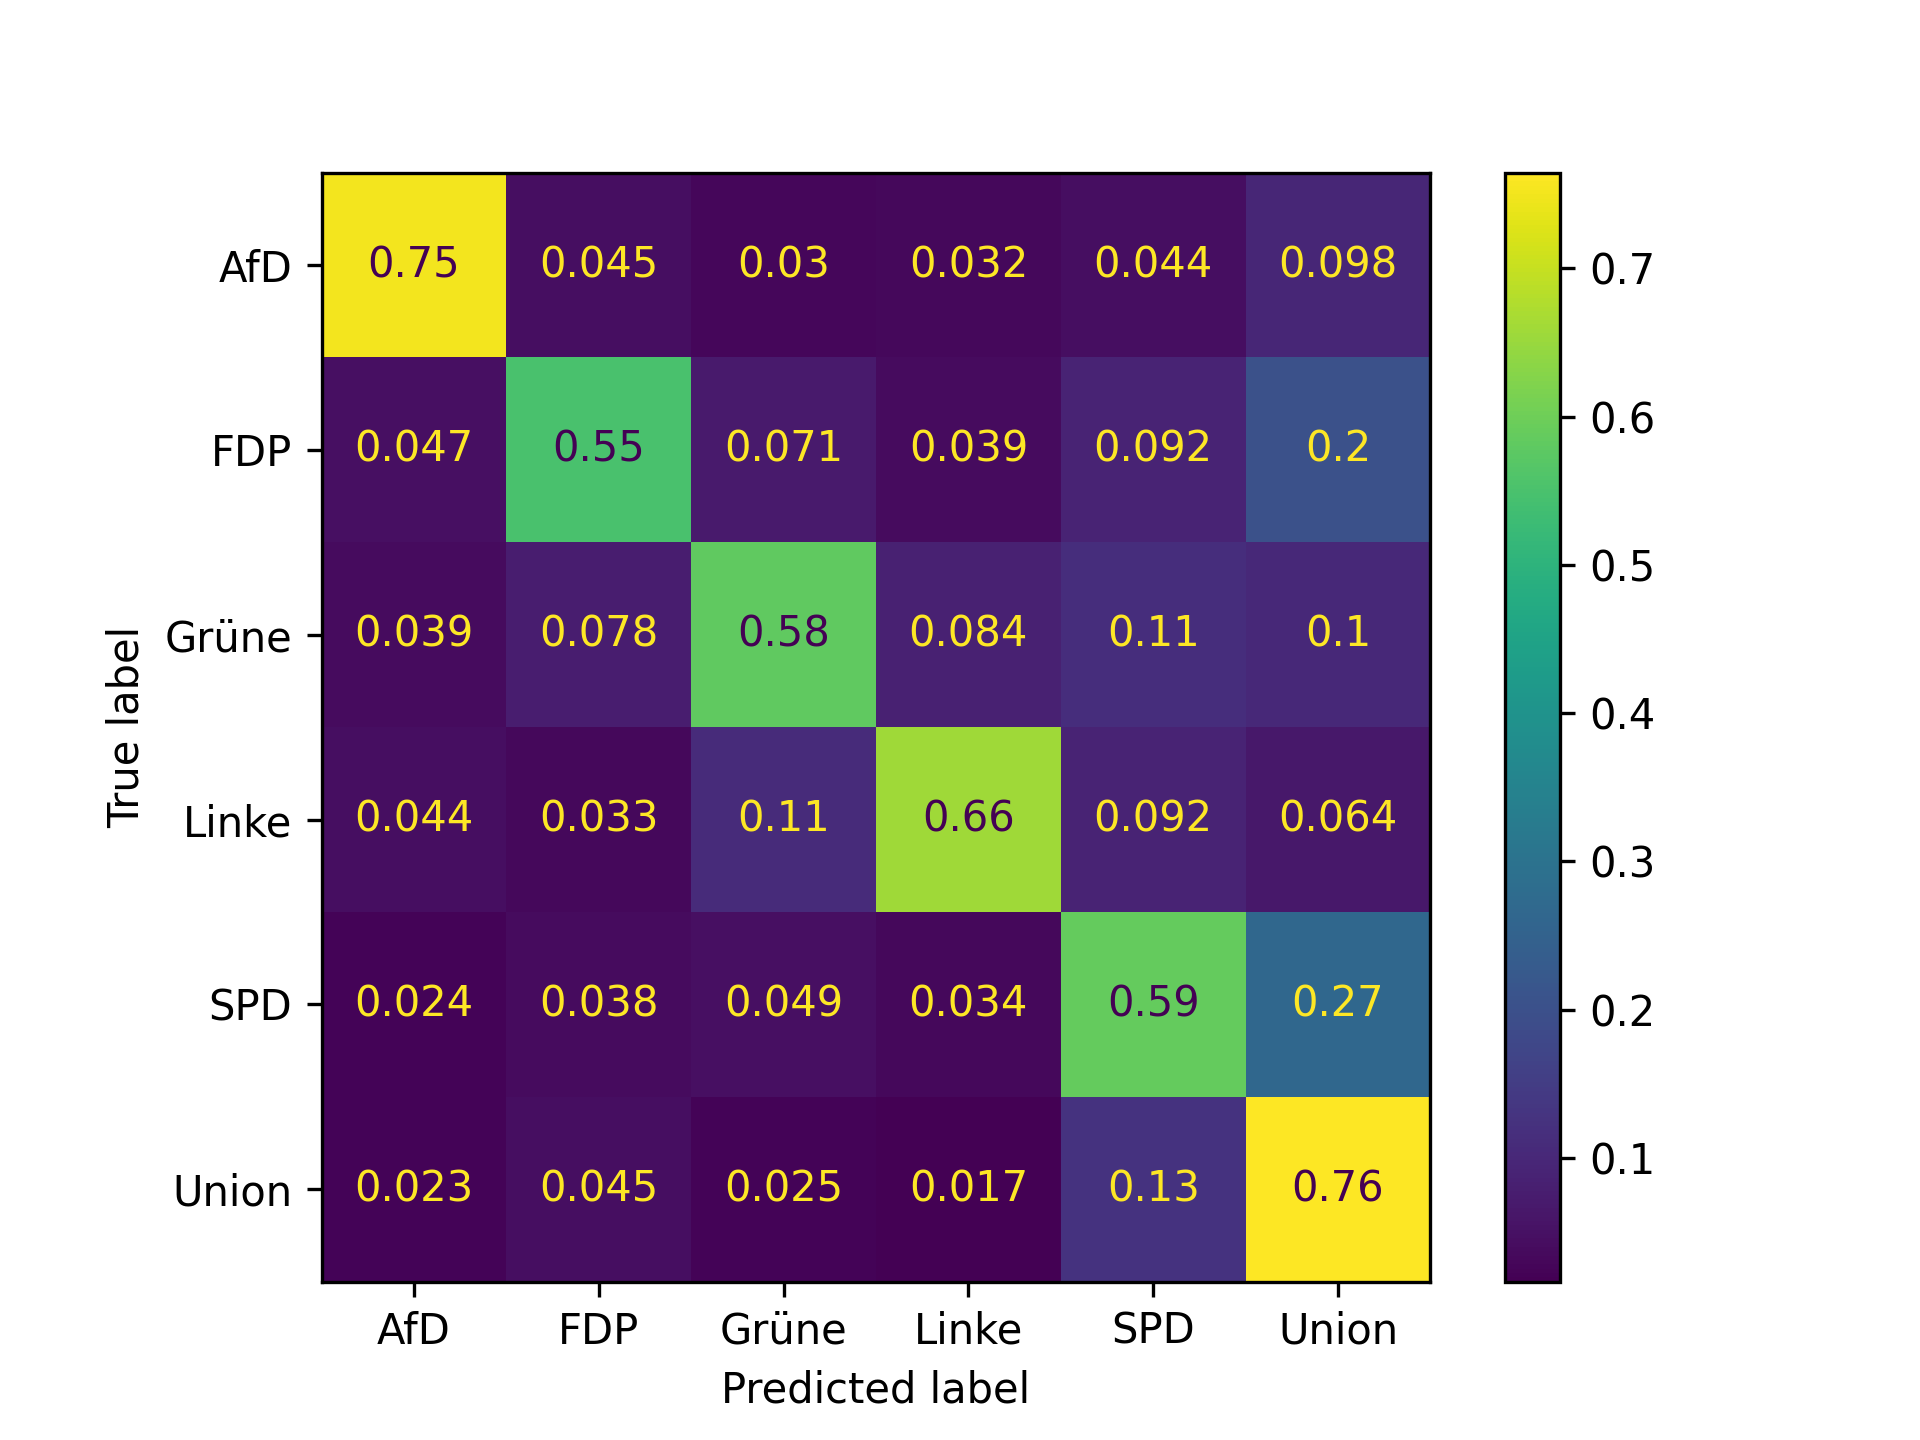
\includegraphics[width=\textwidth]{data/images/modeling/mlp/speeches_confusion_matrix.png}
    \caption{Reden (\(N=\num{38475}\)), \ac{BoW}}
    \label{sfig:confusionMatrixMlpSpeeches}
\end{subfigure}
\caption[Konfusionsmatrizen für das \acs{MLP}-Modell auf unausgeglichenen Datensätzen]{Konfusionsmatrizen für das \acs{MLP}-Modell auf unausgeglichenen Datensätzen. $N$ repräsentiert die Anzahl an Trainings- und Testdaten.} \label{fig:confusionMatrixMlp}
\end{figure}

\subsection{CNN}

\begin{figure}[H]
  \centering
  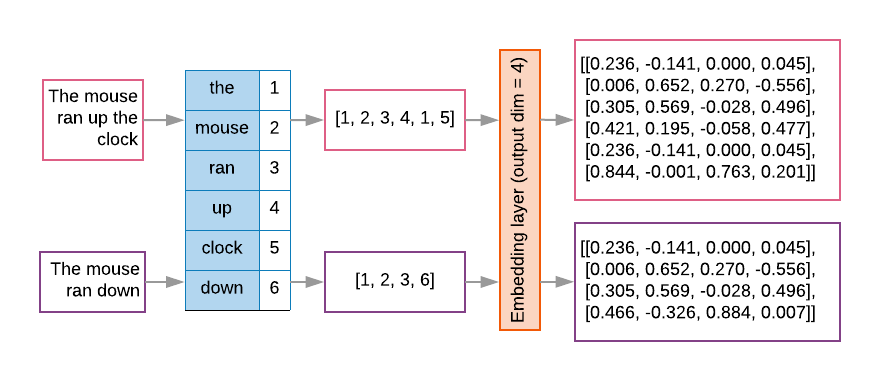
\includegraphics[width=0.8\textwidth]{data/images/embedding_layer.png}
  \caption{Funktionsweise der Embedding-Schicht} \label{fig:embeddingLayer}
\end{figure}

\begin{figure}[H]
  \centering
  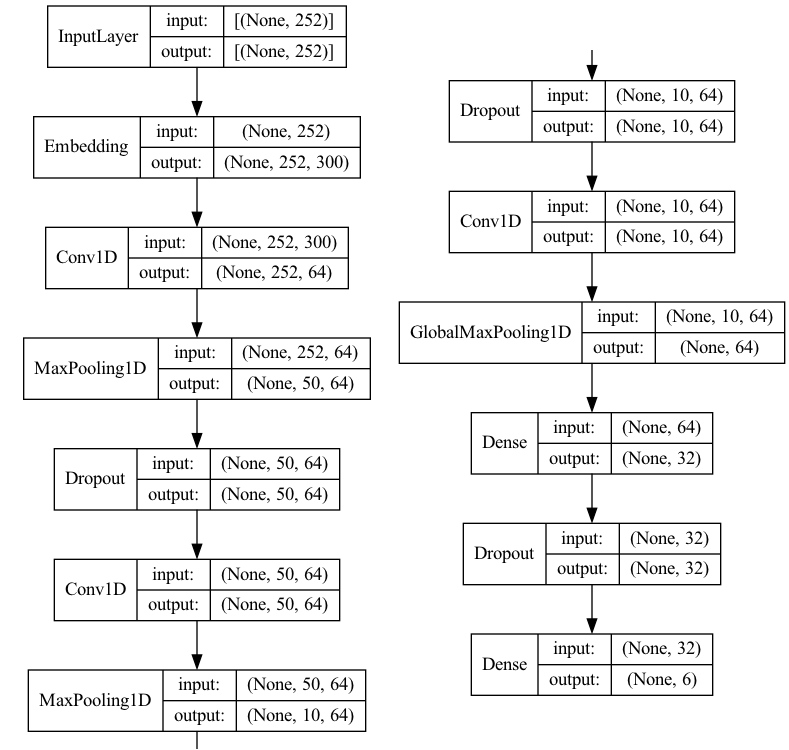
\includegraphics[width=0.6\textwidth]{data/images/cnn.png}
  \caption{Übersicht über die \acs{CNN}-Archtitektur} \label{fig:cnnArchitecture}
\end{figure}

{\footnotesize
\begin{longtblr}[caption={Makro \(F_1\) Score für \acs{CNN}-Modell}, label={tab:overviewScoresCNN}, remark{Parameter} = {\(E = \num{20}\), \(LR = \num{7.5e-4}\), \(B = \num{64}\)}]{width=\textwidth, hline{1-2, Z} = {1pt}, colspec={l*{2}{Q[si={table-format=1.2},c]}}, row{1}={guard,font=\bfseries,l}}
    Datensatz & Unbalanced & Balanced \\ 

    Tweets & \textbf{\num{0.46}} & 0.44 \\
    Wahlprogramme & \textbf{\num{0.48}} & 0.44 \\ 
    Reden & \textbf{\num{0.58}} & 0.53 \\ 
    \hline
    Kombiniert & \textbf{\num{0.48}} & 0.47 \\ 
\end{longtblr}
}

\begin{figure}[H]
    \centering
    \begin{subfigure}{0.49\textwidth}
        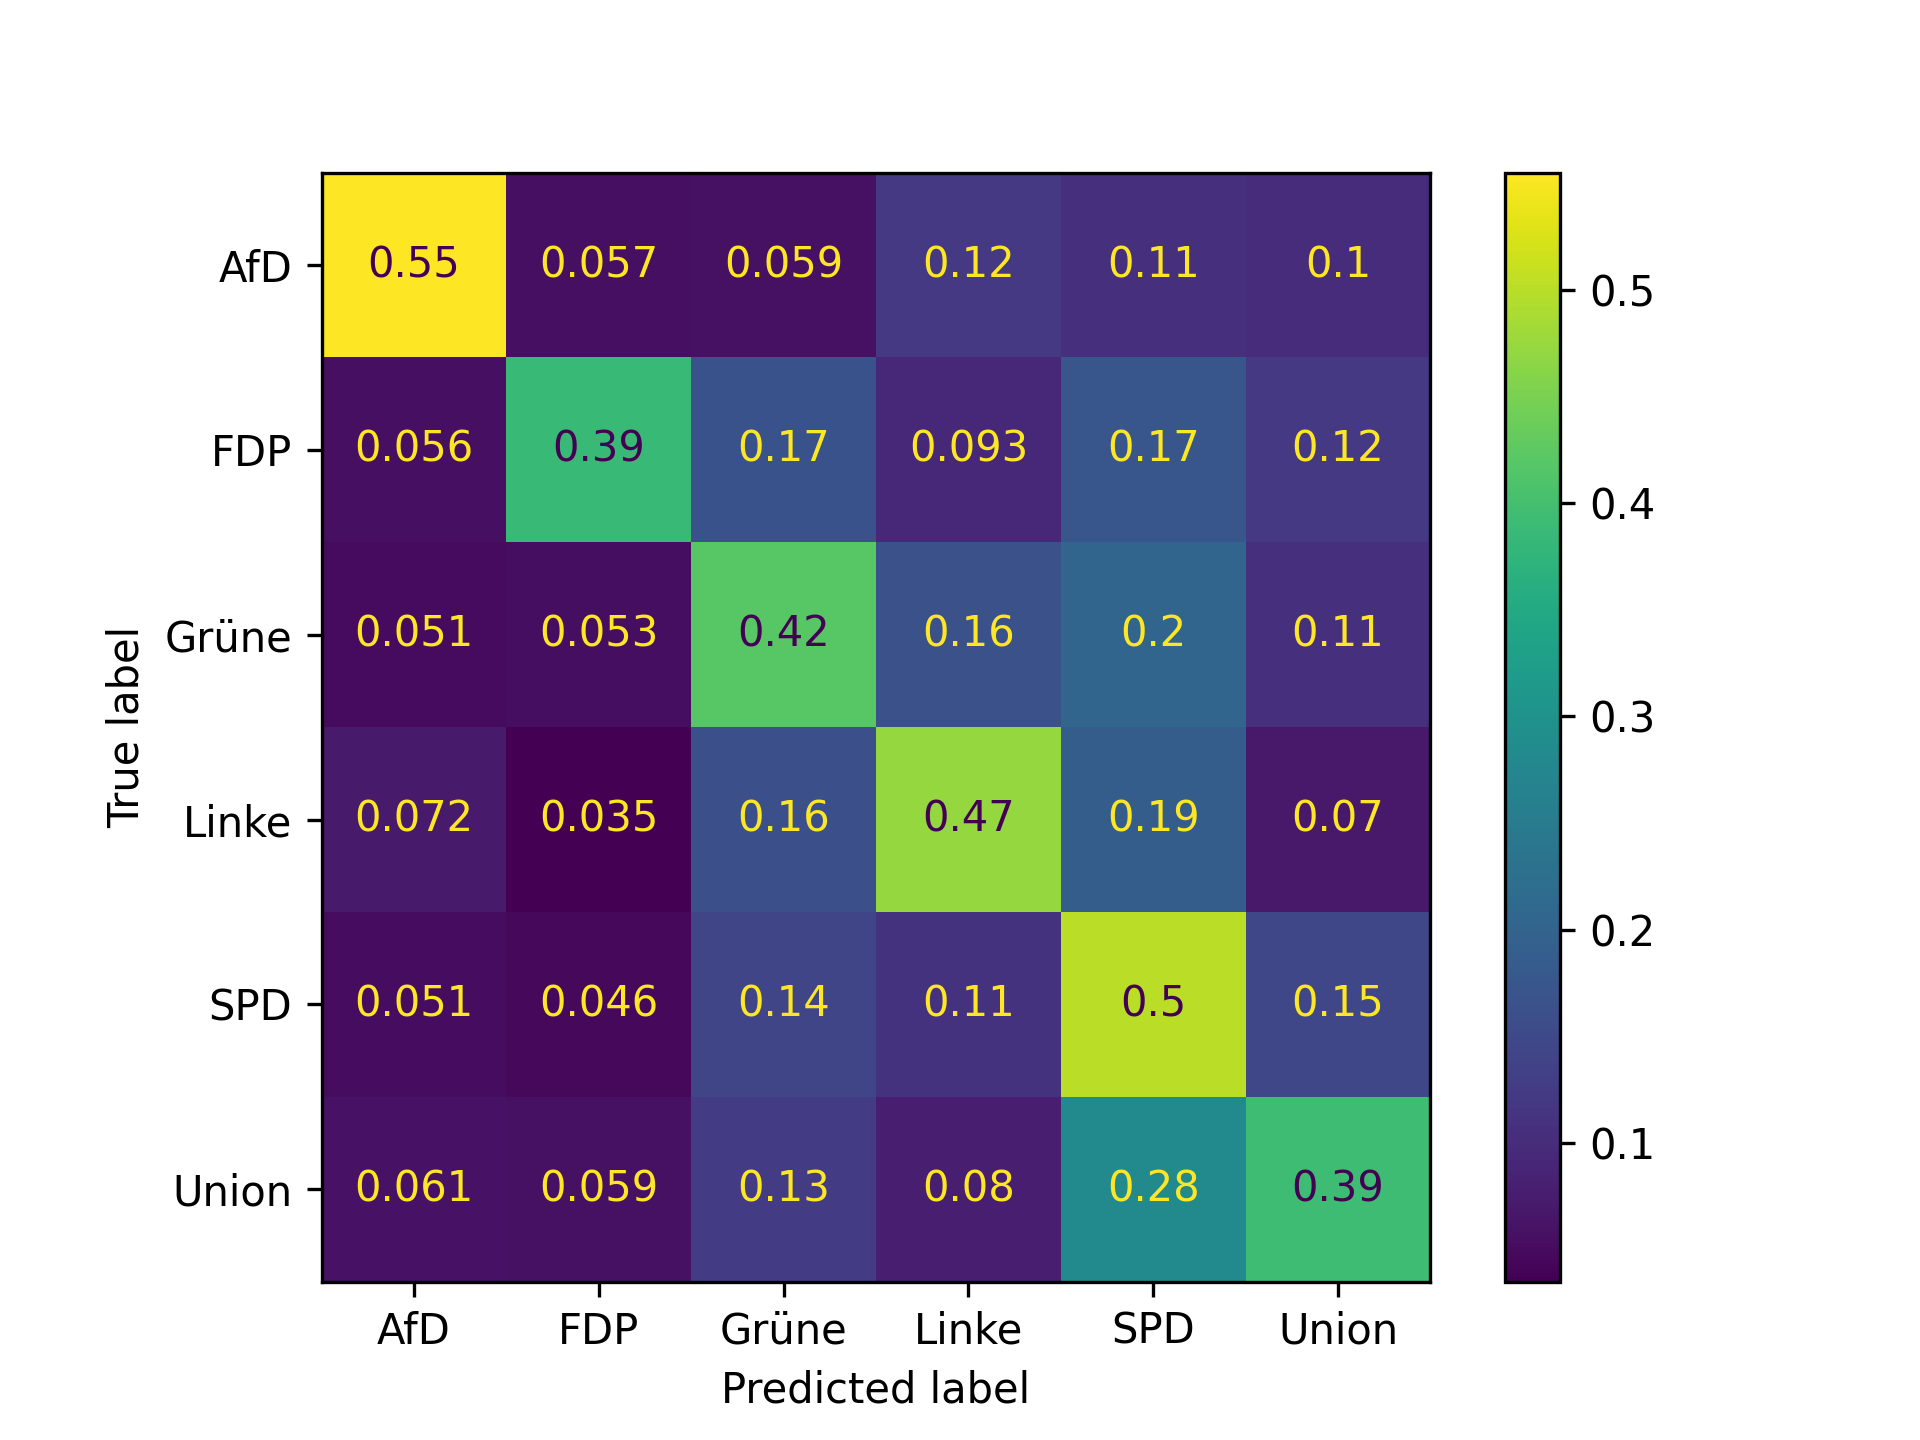
\includegraphics[width=\textwidth]{data/images/modeling/cnn/tweets_confusion_matrix.png}
        \caption{Tweets (\(N=\num{326625}\))}
        \label{sfig:confusionMatrixCnnTweets}
    \end{subfigure}
    \hfill
    \begin{subfigure}{0.49\textwidth}
        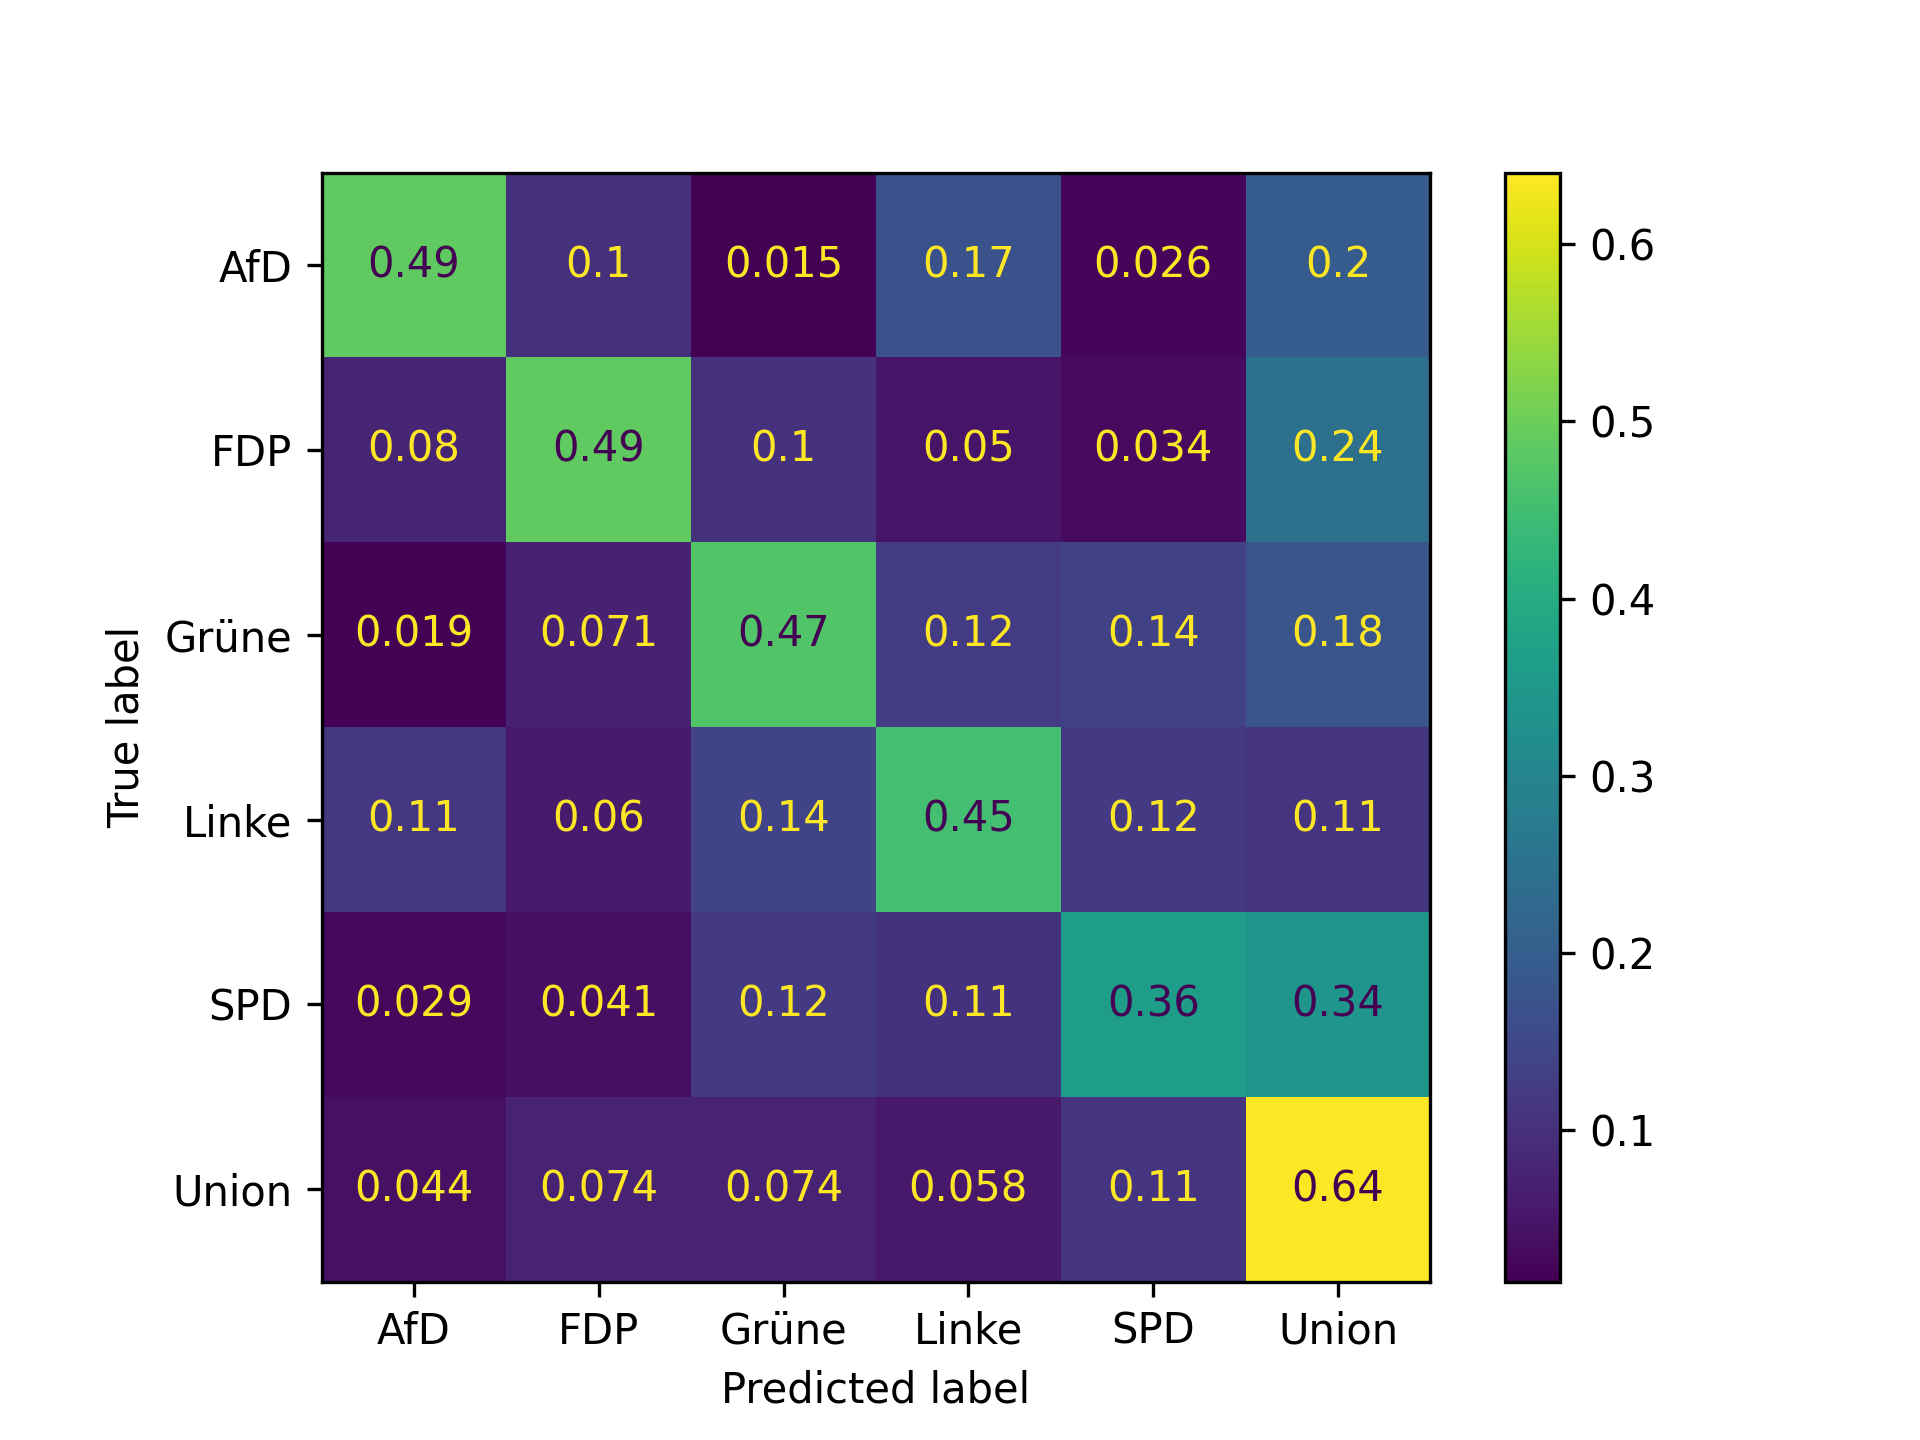
\includegraphics[width=\textwidth]{data/images/modeling/cnn/party_programs_confusion_matrix.png}
        \caption{Wahlprogramme (\(N=\num{27674}\))}
        \label{sfig:confusionMatrixCnnManifest}
    \end{subfigure}
    \hfill
    \begin{subfigure}{0.49\textwidth}
        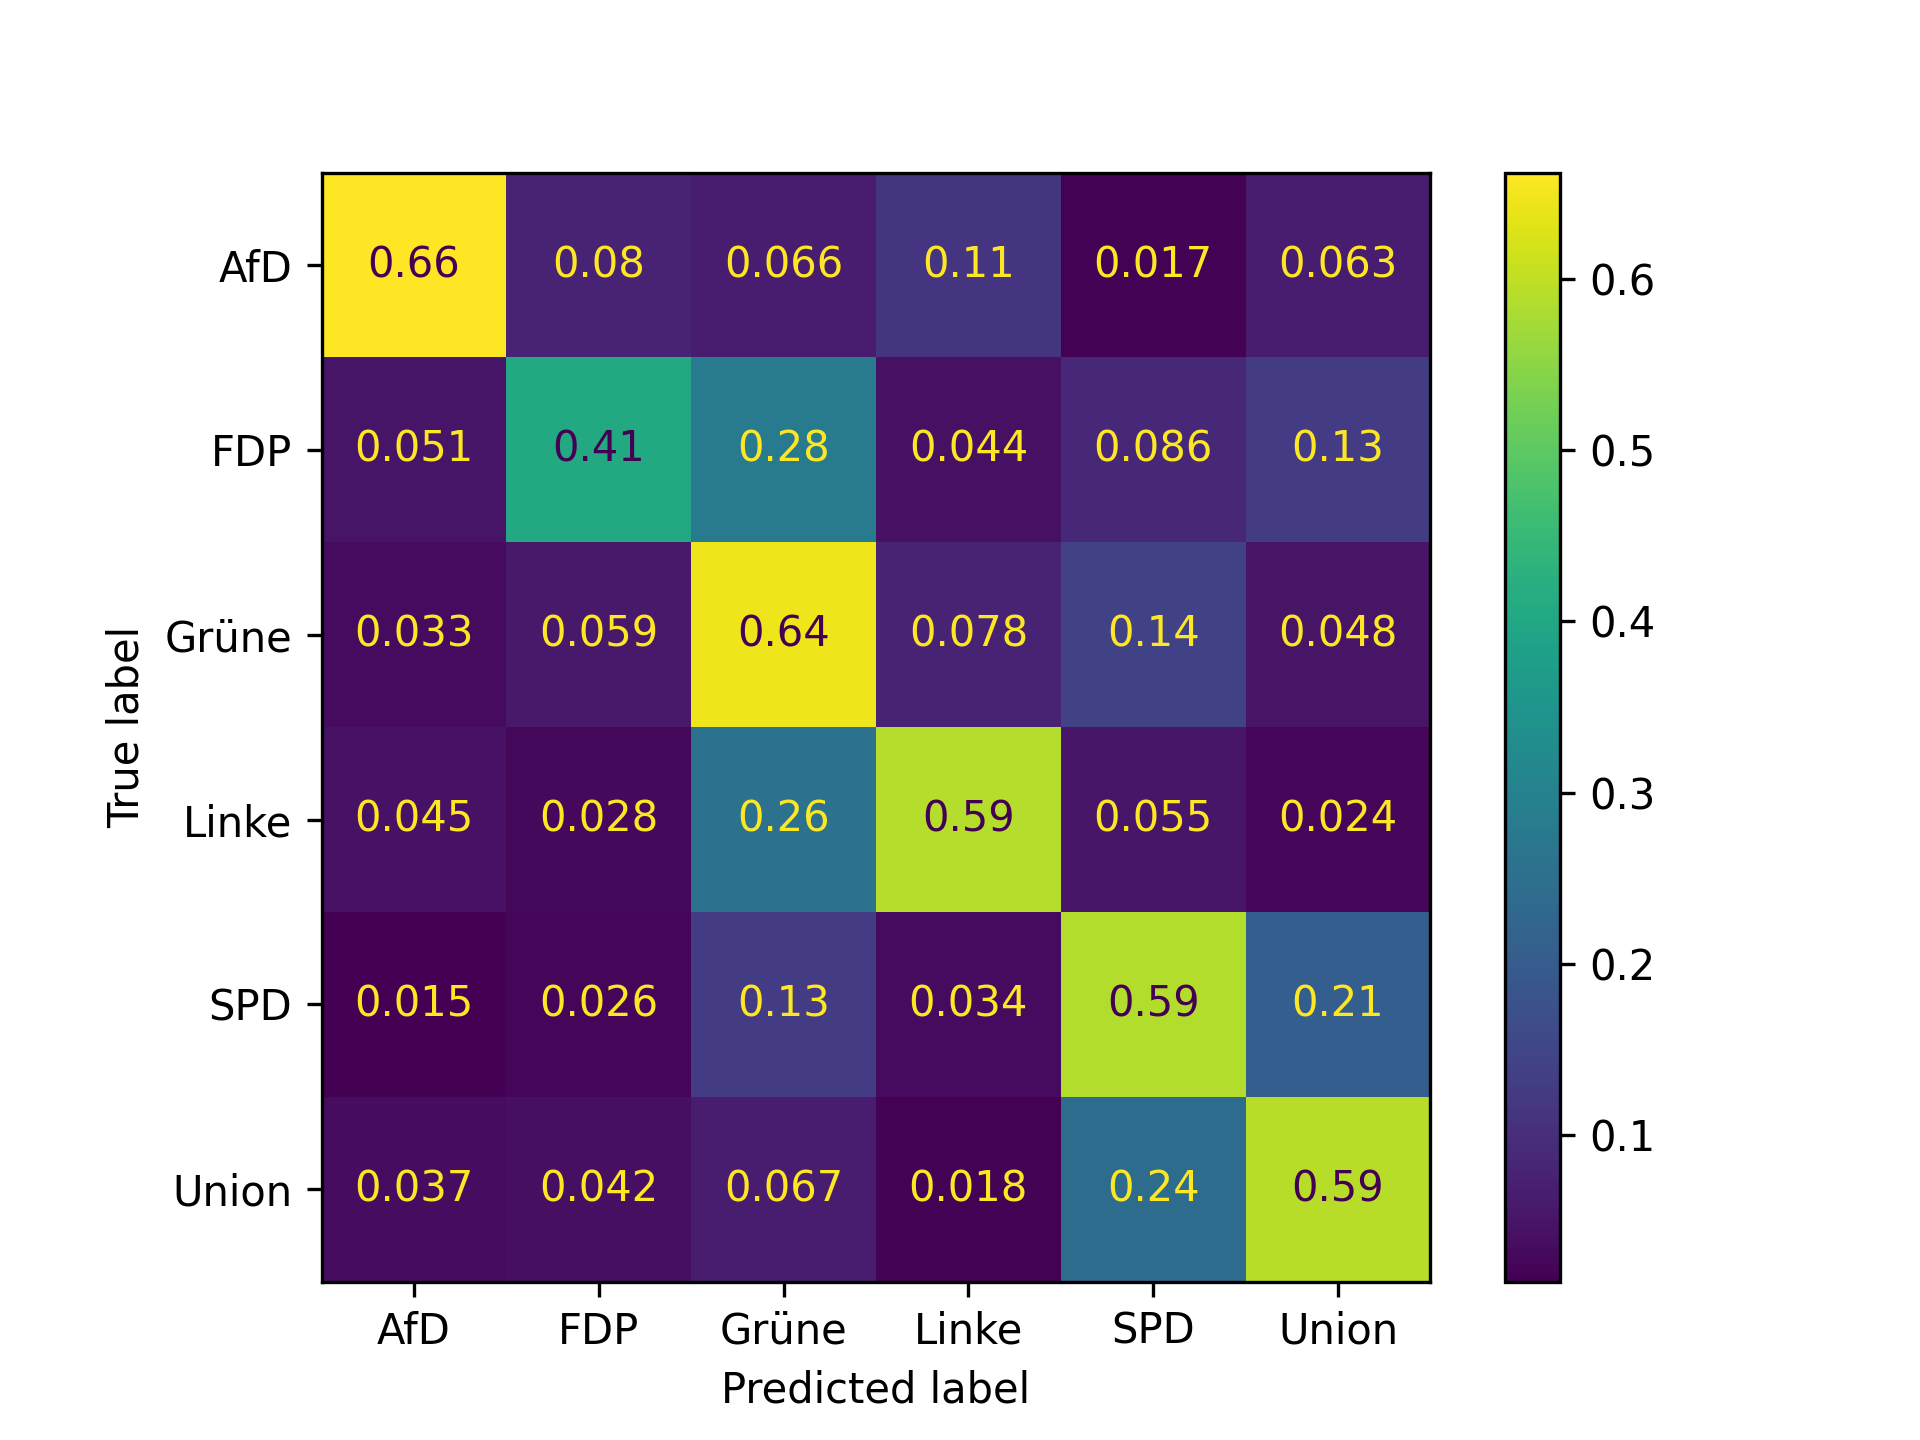
\includegraphics[width=\textwidth]{data/images/modeling/cnn/speeches_confusion_matrix.png}
        \caption{Reden (\(N=\num{38475}\))}
        \label{sfig:confusionMatrixCnnSpeeches}
    \end{subfigure}
    \hfill
    \begin{subfigure}{0.49\textwidth}
        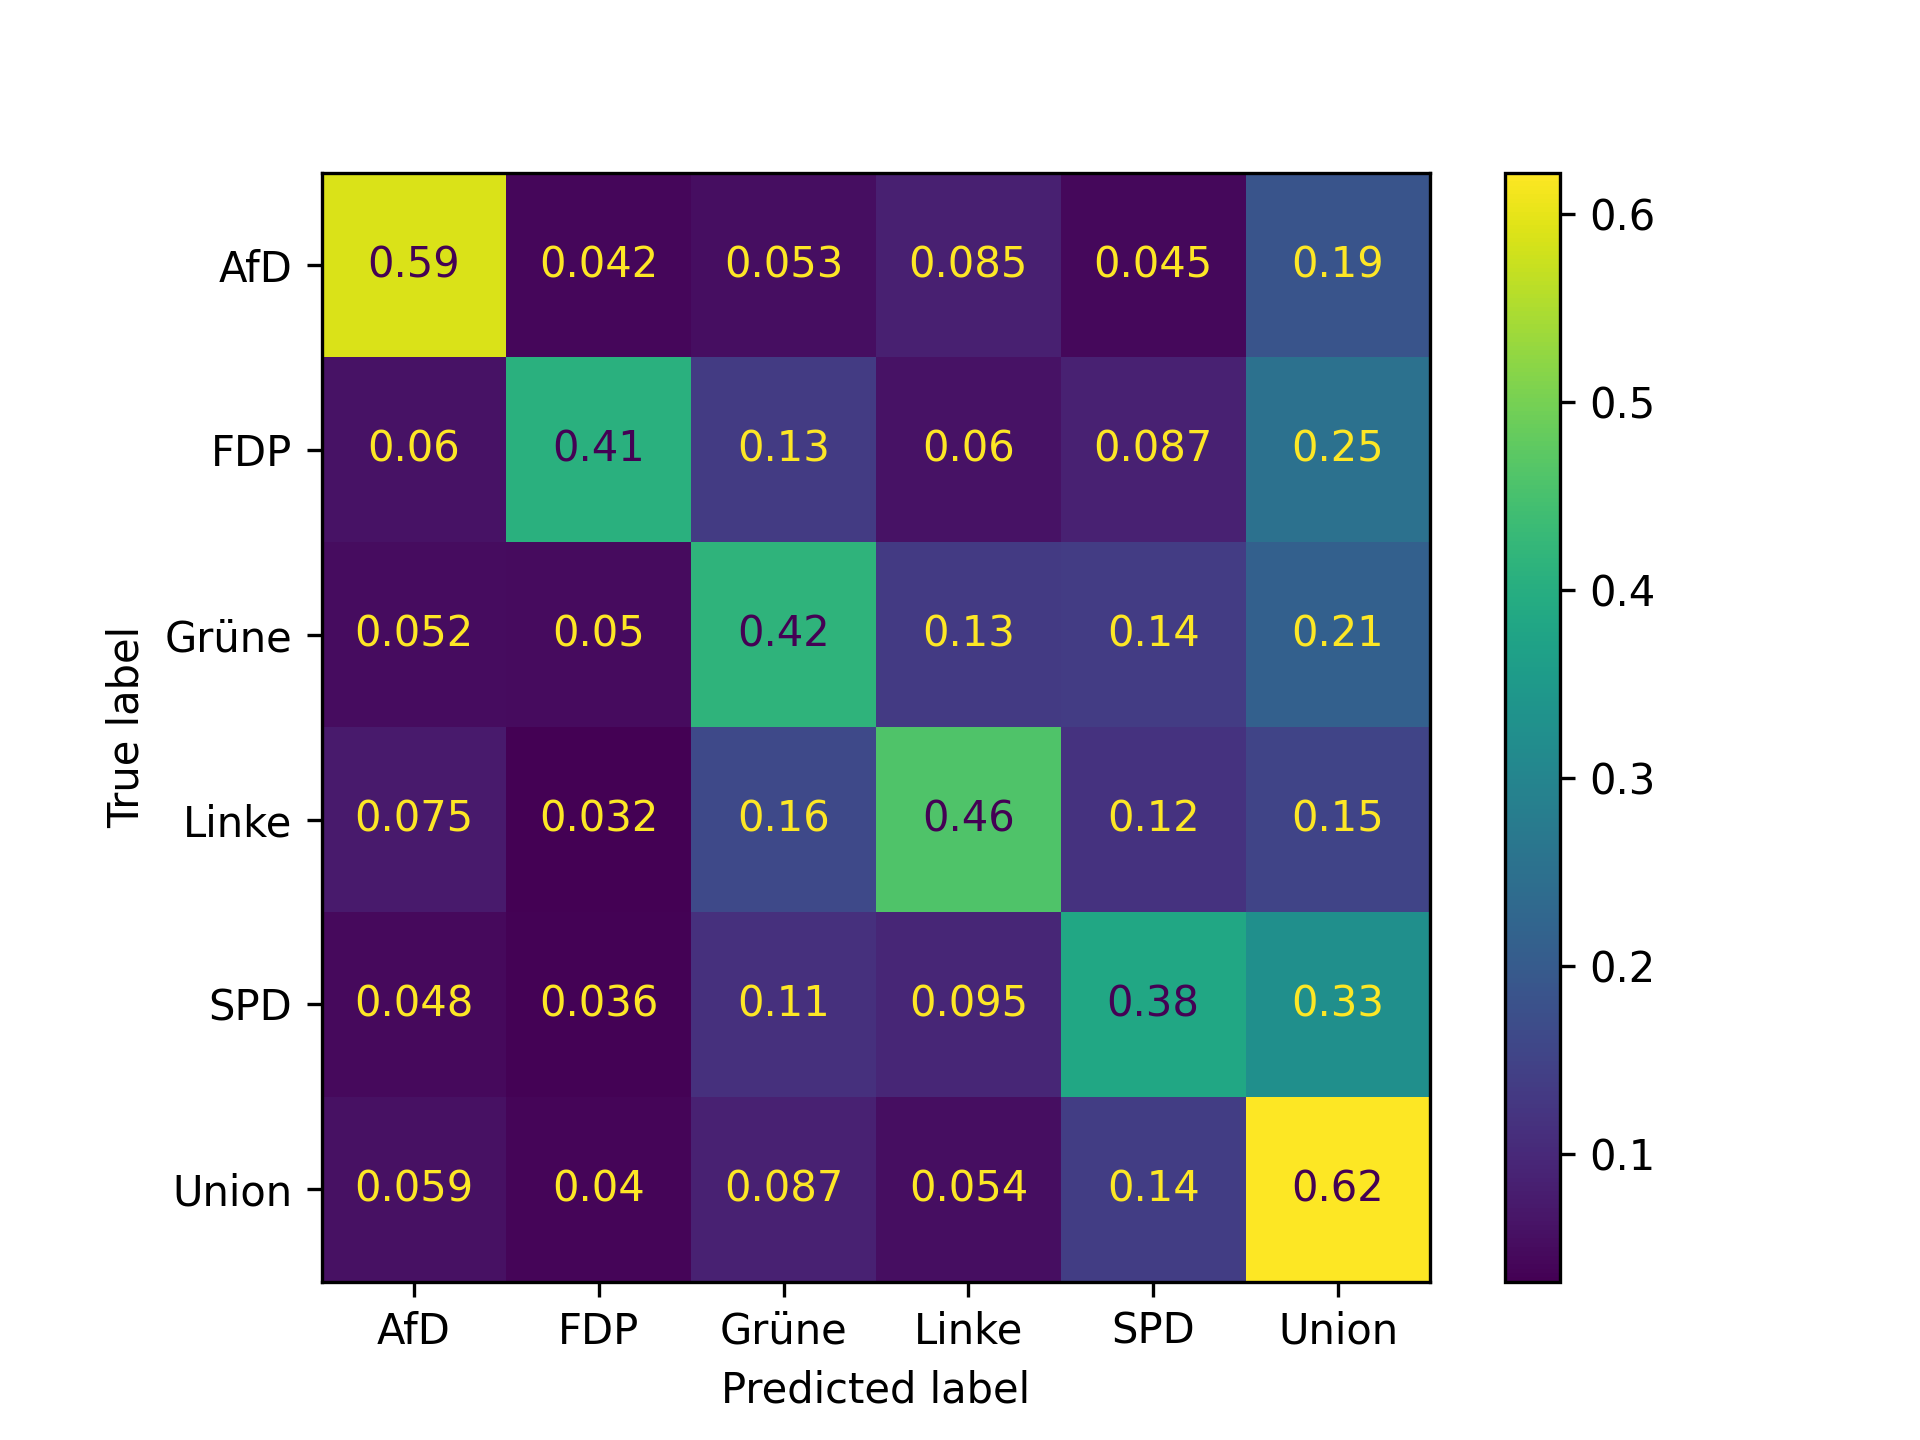
\includegraphics[width=\textwidth]{data/images/modeling/cnn/all_confusion_matrix.png}
        \caption{Kombinierter Datensatz (\(N=\num{392774}\))}
        \label{sfig:confusionMatrixCnnAll}
    \end{subfigure}
    \caption[Konfusionsmatrizen für das \ac{CNN}-Modell auf unausgeglichenen Datensätzen]{Konfusionsmatrizen für das \ac{CNN}-Modell auf unausgeglichenen Datensätzen. $N$ repräsentiert die Anzahl an Trainings- und Testdaten.} \label{fig:confusionMatrixCnn}
\end{figure}

\subsection{BERT}

In diesem Abschnitt werden die Ergebnisse für das Training mit \ac{BERT} präsentiert. Für dieses werden zwei vortrainierte Modelle verwendet. Zum einen \href{https://huggingface.co/dbmdz/bert-base-german-uncased}{\texttt{dbmdz/bert-base-german-uncased}} (veröffentlicht unter \dots) und \href{https://huggingface.co/distilbert-base-german-cased}{\texttt{distilbert-base-german-cased}} (veröffentlicht unter Apache-Lizenz Version 2.0). 

Für die Learning-Rate wird der gleiche Wert von \num{2e-5} wie bei \textcite{guhr_training_2020} angenommen. Die Batch-Size wird abhängig vom Datensatz variiert, da unter anderem die Tweets deutlich kürzer sind als vergleichsweise einzelne Wahlprogramm-Paragraphen. Dadurch benötigen diese weniger Speicherplatz auf der \ac{GPU}.

{\footnotesize
\begin{longtblr}[caption={Makro \(F_1\) Score für \ac{BERT} Modelle}, label={tab:overviewScoresBert}, remark{Parameter} = {\(E = \num{3}\), \(LR = \num{2e-5}\), \(8 \leq B \leq 32\)}, note{$\dag$}={\ac{GDDR5} Speicher reicht nicht für das Training.}]{hline{1, 3, Z} = {1pt}, rowhead = 2, colspec={l*{4}{Q[si={table-format=1.2},c]}}, row{1-2}={guard,font=\bfseries,l}}
     & \SetCell[c=2]{c} BERT & & \SetCell[c=2]{c} DistilBERT & \\ 
    \cline{2-5}
    Datensatz & Unbalanced & Balanced & Unbalanced & Balanced \\ 

    Tweets & \textbf{\num{0.62}} & 0.59 & 0.58 & 0.56 \\*
    Wahlprogramm & \textbf{\num{0.66}} & 0.61 & 0.62 & 0.58 \\*
    Reden & \textbf{\num{0.72}} & 0.66 & 0.67 & 0.65 \\*
    \hline
    Kombiniert & 0\TblrNote{$\dag$} & 0\TblrNote{$\dag$} & \textbf{\num{0.60}} & 0.58 \\
\end{longtblr}
}

% distilbert-base-german-cased:
 % Tweets (00h00min, lr 2-e5, epochs 3, batch 64) &
 % Wahlprogramm (
 % Reden (1h24min, lr 2-e5, epochs 3, batch 16) &

\section{Evaluation} \label{sec:evaluation}

% TODO: Einleitung hinzufügen

\subsection{Weitere Experimente} \label{subsec:furtherExperiments}

\subsubsection{Out-of-domain}

% TODO: Klassifikationsergebnisse von exemplarisch ausgewählten Texten unterschiedlicher Art zwischen mehreren Modellen (die auf anderen Datensätze basieren) vergleichen. Welchen Einfluss haben die verwendeten Daten darauf, was für eine Art von Text jeweils einer Partei besonders stark zugeordnet oder als neutral eingeordnet wird?

Bei jeglicher Form von \ac{ML} Modellen stellt sich die Frage, wie allgemeingültig das jeweilige Modell angewendet werden kann. Wie in \autoref{sec:thesisGoal} formuliert, soll dies ebenfalls für eine Auswahl an Modellen aus dieser Arbeit überprüft werden. Ähnlich zu \textcite{biessmann_predicting_2016} werden hierfür Modelle verwendet, welche lediglich auf einen der drei Datensätze trainiert wurden. Anschließend werden alle unbalancierten Datensätze auf Basis es gewählten Modells validiert. Als Bewertungsmetrik wird der Makro $F_{1}$ Score verwendet.

{\footnotesize
\begin{longtblr}[caption={Out-of-domain Makro \(F_1\) Score für \ac{BERT} und \ft Modelle}, label={tab:overviewScoresOutDomain}, remark{Anmerkung}={Validierung erfolgt auf den gesamten, unbalancierten Datensätzen}, note{$\dag$}={In-domain}]{hline{1, 3, Z} = {1pt}, rowhead = 2, colspec={l*{6}{Q[si={table-format=1.2},c]}}, row{1-2}={guard,font=\bfseries,l}}
     & \SetCell[c=3]{c} BERT & & & \SetCell[c=3]{c} DistilBERT & & \\ 
    \cline{2-7}
    Datensatz & Tweets & Reden & Wahlprogramme & Tweets & Reden & Wahlprogramme \\ 

    Tweets & 0.0\TblrNote{$\dag$} & 0.0 & 0.0 & 0.0\TblrNote{$\dag$} & 0.0 & 0.0 \\*
    Wahlprogramm & 0.0 & 0.0\TblrNote{$\dag$} & 0.0 & 0.0 & 0.0\TblrNote{$\dag$} & 0.0 \\ *
    Reden & 0.0 & 0.0 & 0.0\TblrNote{$\dag$} & 0.0 & 0.0 & 0.0\TblrNote{$\dag$} \\ 
\end{longtblr}
}

\subsubsection{Erweiterter Zeitraum}

\begin{table}[H]
    \centering
    \caption{Makro \(F_1\) Score für Reden verschiedener Zeiträume} \label{tab:overviewScoresExtendedPeriod}
    {\footnotesize
    \begin{tblr}{width=\textwidth, hline{1-2, Z} = {1pt}, colspec={c*{2}{Q[si={table-format=1.2},c]}}, row{1}={guard,font=\bfseries,l}}
        Wahlperiode & \ft & Lineare SVC \\ 

        \num{19} & 0.72 & 0.69 \\
        \numrange{18}{19} & 0.69 & 0.65 \\ 
        \numrange{17}{19} & 0.66 & 0.61 \\ 
        \numrange{16}{19} & 0.64 & 0.60 \\ 
    \end{tblr}
    }
\end{table}

\subsubsection{Sentence Level}

{\footnotesize
\begin{longtblr}[caption={Makro \(F_1\) Score für Sentence-Level Daten}, label={tab:overviewScoresSentenceLevel}, remark{Parameter \ft} = {\(E = \num{20}\), \(LR = \num{0.1}\)}, remark{Note} = {Aufgrund der Länge und nicht eindeutigen Satzstrukturen werden Tweets nicht in Sätze unterteilt.}]{hline{1, 3, Z} = {1pt}, rowhead = 2, colspec={l*{4}{Q[si={table-format=1.2},c]}}, row{1-2}={guard,font=\bfseries,l}}
     & \SetCell[c=2]{c} \ft & & \SetCell[c=2]{c} CNN & \\ 
    \cline{2-5}
    Datensatz & Unbalanced & Balanced & Unbalanced & Balanced \\ 

    Wahlprogramme & \textbf{\num{0.41}} & 0.36 & 0.33 & 0.31 \\
    Reden & \textbf{\num{0.33}} & 0.31 & 0.24 & 0.27 \\
    \hline
    Kombiniert & \textbf{\num{0.41}} & 0.38 & 0.26 & 0.29 \\
\end{longtblr}
}

\subsection{Diskussion} \label{subsec:discussion}

\subsubsection{Klassifikation von Polysemie}

% TODO: Add example for polysemy

Durch Methoden wie \ac{BoW} und \ac{TF-IDF} gehen syntaktische, als auch semantische Zusammenhänge verloren \autocite[48\psq]{kowsari_text_2019}. Das führt dazu, dass Modelle wie \ac{SVM} und Random Forest ausschließlich die verwendeten Wörter und deren Anzahl in Betracht zieht, aber nicht die tiefere Bedeutung im Kontext des Satzes. Nach \textcite{kowsari_text_2019} versuchen Modelle wie Word2Vec, GloVe und \ft zumindest syntaktische und semantische Zusammenhänge zu berücksichtigen, jedoch haben selbst diese Modelle Schwierigkeiten, Polysemie\footnote{Sätze mit mehreren Bedeutungen} zu klassifizieren.

% TODO: BERT

\subsubsection{Neutralität von Texten} % Sprache, Anzahl an Klassen und fehlende neutrale Klasse

% TODO: Add sources and examples

Des Weiteren ergibt sich aus der Wahl der Datenquellen (Wahlprogramme, Reden und Tweets) eine Annahme/Voraussetzung/Bias geben über der verwendeten Sprache. Wahlprogramme, Reden und Tweets von Politikern weisen zwar parteispezifische Wörter auf, jedoch ist die semantische und syntaktische Komplexität der Sätze überdurchschnittlich hoch. Ebenfalls ist die Menge an Rechtschreibfehlern und verwendetem Slang geringer als bei anderen Textarten. Daraus folgt, dass die Performance der trainierten Modelle voraussichtlich signifikant schlechter ist, wenn Texte sprachlich (semantisch und syntaktisch) stark von den Trainingsdaten abweichen.

Inmitten dieses Projektes hat sich die Frage aufgetan, ob zusätzlich zu den sechs Klassen (Linke, ..., Union) ebenfalls eine neutrale, oder nicht klassifizierbare Klasse hinzugefügt werden sollte. Ähnlich zu der Arbeit von \textcite{guhr_training_2020} wo nicht nur positiver und negativer Sentiment analysiert wird, sondern ebenfalls neutral. Dies hat den Hintergrund, dass es ebenfalls Texte gibt, welche keine eindeutig polarisierende Semantik aufweisen. Der gleiche Gedanke lässt sich ebenfalls auf ein politisches Klassifikationsmodell anwenden. Textquellen wie Wikipedia oder fachliche Artikel weisen womöglich eine neutrale, unpolitische Haltung auf. Eine Klassifikation dieser würde irreführend sein. Ein möglicher Lösungsansatz zur Erweiterung der in \autoref{sec:dataUnderstanding} wäre das Hinzufügen von neuralen Texten wie bei \textcite{guhr_training_2020}.

% TODO: Bezug zu analysen in in-domain herstellen

\subsubsection{Politische Nähe}

% TODO: Add sources and image
% TODO: Reason --> Politisches Viereck (links -- rechts, ...)

Parteien, die ähnliche politische Ideale verfolgen, identische Themenschwerpunkte haben, lassen sich schlechter klassifizieren.

Regierungsparteien und Opposition weisen jeweils höhere falsch Klassifikationen auf.

\subsubsection{Begrenztes Vokabular}

Da Bow und Tf-Idf lediglich auf den drei Datensätzen trainiert wird, lässt sich ebenfalls nur dieses Vokabular vorhersagen.

Vortrainierte Worteinbettungen sind auf allgemeinen Texten trainiert. Zwischen dem Wortschatz und der Semantik von Wörtern kann daher eine Diskrepanz vorliegen, die zu schlechteren Ergebnissen führt. (Word2Vec, GloVe)
\ft lässt ebenfalls die Klassifikation von untrainierten Wörtern zu.

Vortrainierte BERT Modelle über einen sehr großen Wortschatz verfügen. Dennoch Slang und Rechtschreibfehler schwerer zu klassifizieren

\subsubsection{State-of-the-Art}

\begin{figure}[H]
  \centering
  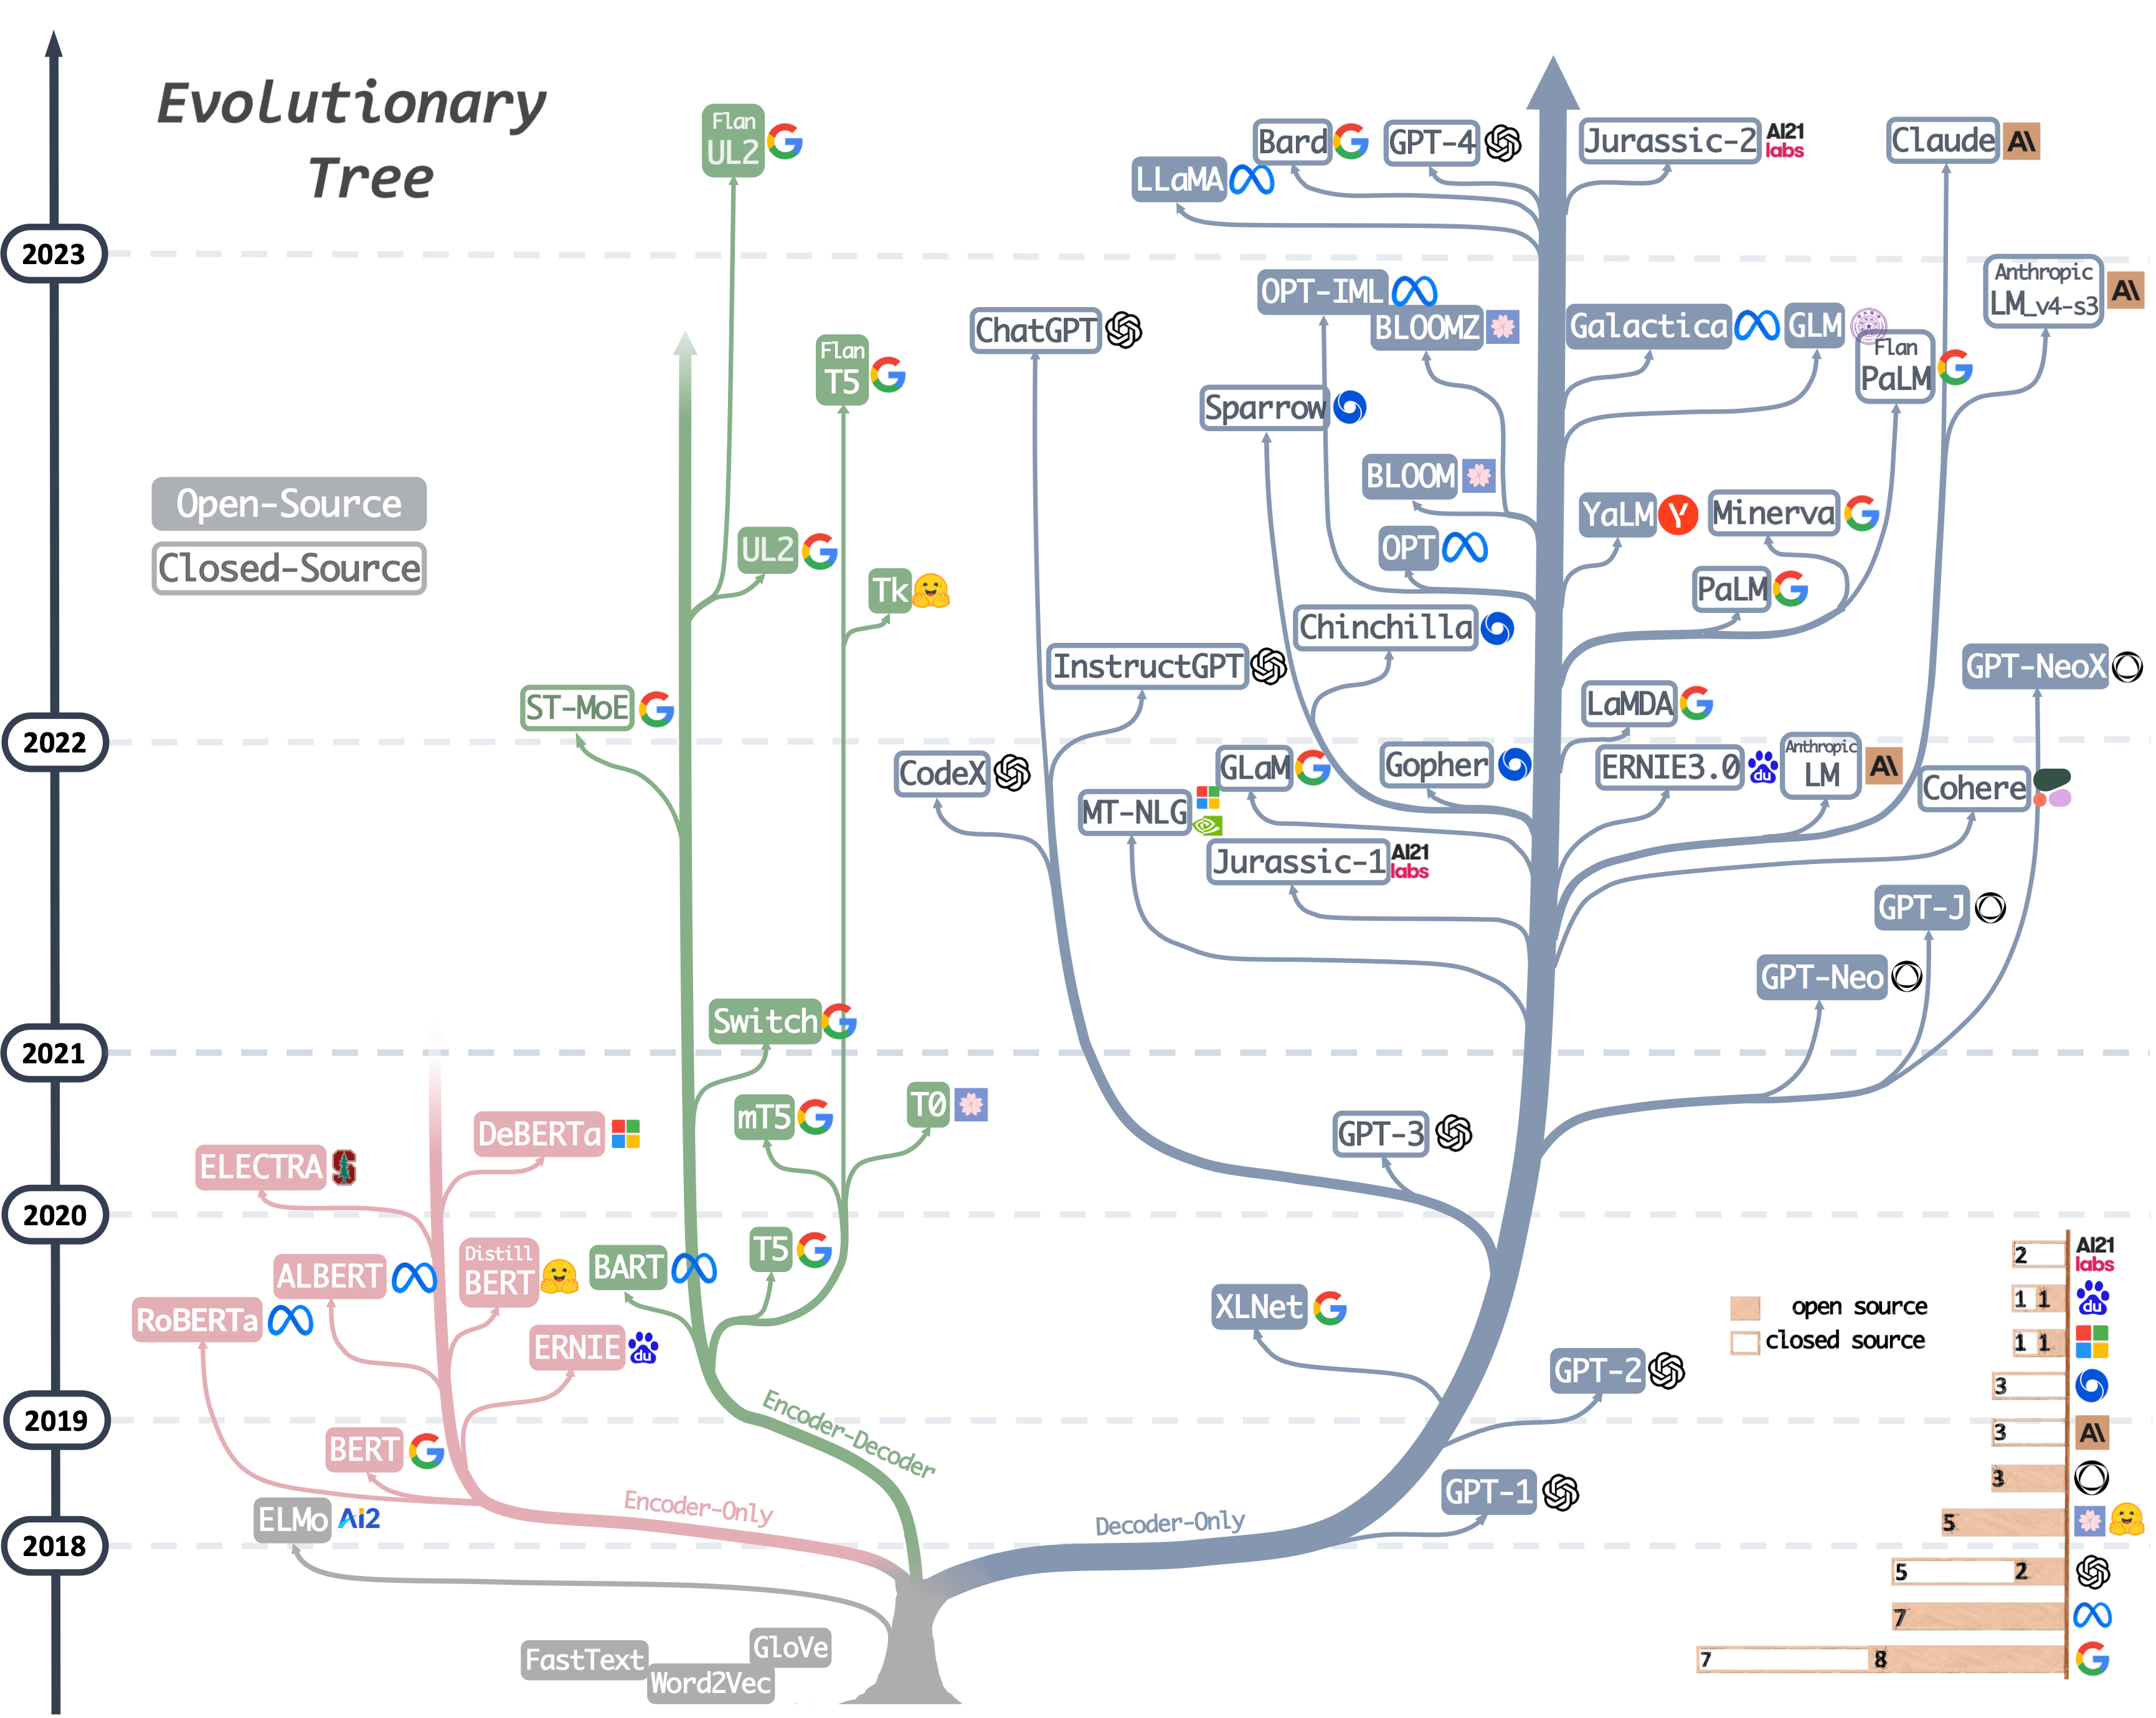
\includegraphics[width=0.7\textwidth]{data/images/tree.png}
  \caption{Übersicht über State-of-the-Art von \acp{LLM} \autocite{yang_harnessing_2023}} \label{fig:stateOfTheArt}
\end{figure}

Modelle nicht state of the art
Häufig Ressourcenlimitationen bei größeren Modellen wie Roberta oder \dots
Andere Modelle häufig closed source
Außerdem sind viele Modelle nicht in deutsch verfügbar

\section{Bereitstellung der Klassifikationsmodelle} \label{sec:crispDm_3}

Hugging Face ist eine Plattform, welche es ermöglicht, \ac{ML} Modelle öffentlich bereitzustellen. Im Rahmen dieser Arbeit wird das \ac{BERT} Modell auf Basis des \texttt{distilbert-base-german-cased} Modells zur Verfügung gestellt. \href{https://huggingface.co/felixhoffmnn/GePart}{DistilBERT}

\section{Fazit} \label{sec:crispConclusion_2}

% TODO: Add Conclusion
